\documentclass{article}
\usepackage[utf8]{inputenc}
\usepackage[T1]{fontenc}
\usepackage{amsmath}
\usepackage{amssymb,amsfonts,textcomp}
\usepackage{array}
\usepackage{hhline}
\usepackage{hyperref}
\hypersetup{colorlinks=true, linkcolor=blue, citecolor=blue, filecolor=blue, urlcolor=blue, pdftitle=, pdfauthor=Gilles Vuidel, pdfsubject=, pdfkeywords=}
\usepackage{graphicx}
\usepackage[top=2.501cm,bottom=2.501cm,left=2.501cm,right=2.501cm,nohead]{geometry}
\usepackage{float}
\usepackage{parskip}
\usepackage{caption}
\makeatletter
\newcommand\arraybslash{\let\\\@arraycr}
\makeatother
% centering figures
\makeatletter
\g@addto@macro\@floatboxreset\centering
\makeatother
\setlength\tabcolsep{1mm}
\renewcommand\arraystretch{1.3}

% saut de page après une section
%\let\oldsection\section
%\renewcommand\section{\clearpage\oldsection}

% saut après itemize
\let\EndItemize\enditemize
\def\enditemize{\EndItemize\medskip}

\begin{document}

\begin{titlepage}

	\centering
	
\includegraphics[scale=0.5]{img/logo.png}\\
	
	\bigskip
	\bigskip
	\bigskip	
	{\Huge
	\bfseries
	Graphab 2.5\\
	\bigskip
	User Manual\\
	}
	\bigskip
	\bigskip
	\bigskip
	\bigskip
	\bigskip
			
	{\Large		
	Céline Clauzel, Jean-Christophe Foltête, Xavier Girardet, Gilles Vuidel\\
	\bigskip
	2019-11-21\\
	}
	
\end{titlepage}

\setcounter{tocdepth}{2}
\tableofcontents

\pagebreak

\section{Introduction}

\subsection{About Graphab}

Graphab is a software application for modeling ecological networks using landscape graphs. It is composed of four modules for:
\begin{itemize}
	\item constructing graphs, including loading initial landscape data and identifying patches and links (Euclidean distances or least-cost paths)
	\item computing connectivity metrics from graphs
	\item integrating graph-based connectivity metrics into species distribution models
	\item visual and cartographic interfacing 
\end{itemize}


\textbf{Warning, projects are not compatible between the versions 1.x and 2.x of Graphab !}

\subsubsection{Authors}

Graphab has been developed by Gilles Vuidel and Jean-Christophe Foltête at \href{http://thema.univ-fcomte.fr/}{ThéMA} laboratory (\href{http://www.univ-fcomte.fr}{University of Franche-Comté} – \href{http://www.cnrs.fr}{CNRS}). Funding has been provided by the French Ministry of Ecology, Energy, Sustainable Development and the Sea (\href{http://www.ittecop.fr/}{ITTECOP} Program). The Graphab logo was designed by \href{http://www.gachwell.com/}{Gachwell}.

\subsubsection{Terms of use}

Graphab is distributed in open source, under the GPL license. Users must cite the following reference \cite{2012_graphab_EMS} in their publications:\\
Foltête J.C., Clauzel C., Vuidel G., 2012. A software tool dedicated to the modelling of landscape networks, Environmental Modelling \& Software, 38: 316-327.


\subsection{System requirements}

Graphab runs on any computer supporting Java 8 or later (PC under Linux, Windows, Mac, etc.). However, when dealing with very large datasets, the amount of RAM memory in the computer will limit the maximum number of nodes and links that can be processed in a single run with Graphab. In addition, for some complex metrics, processing power (CPU) will determine the speed of computing. For details, see section \nameref{limit} below and the journal article  \cite{2012_graphab_EMS}.

\subsection{Installing the software and launching a project}

Graphab can be downloaded from \url{https://sourcesup.renater.fr/graphab}.

\begin{itemize}
	\item Download and install Java 8 or later - \href{http://www.java.com}{java.com}. If you have a 64-bit operating system, it is best to install the 64-bit version of Java.
	\item Download graphab-2.4.jar
	\item Launch graphab-2.4.jar
\end{itemize}
After launching graphab-2.4.jar, the File menu provides access to four sections:
\begin{itemize}
	\item File / New project: to create a new project in which all data and results are saved automatically.  
	\item File / Open project: to open an existing project.
	\item File / Preferences: to change certain software parameters: English/French; maximum amount of memory to use; number of processors to use. It is recommended to adjust the amount of memory and number of processors to suit your computer (see section \nameref{limit}).
	\item File / Log window: to display the event log.
\end{itemize}

\section{Starting a Graphab project }

New projects are created from the File / New project menu. The user must complete a series of windows to identify the project, import a landscape map, and create a link set. Each project is associated with a single landscape map but may contain several link sets. After the start phase, the project is the medium for creating multiple graphs and for computing connectivity metrics. 

\subsection{Identifying a project}

In the first window, the user must enter a project name and specify the folder in which it is to be created.

\begin{figure}[H]
	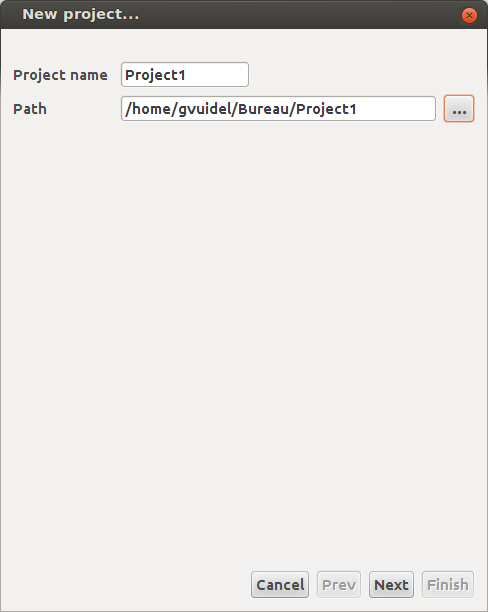
\includegraphics[scale=0.5]{img/manual-en_img2.png}
\end{figure}


\subsection{Importing landscape maps and defining nodes }

The second window is for importing the landscape map. It must be a raster file (*.tif, *.asc, *.rst) in which the value of each pixel corresponds to a category (land cover or other classification).

\begin{figure}[H]
	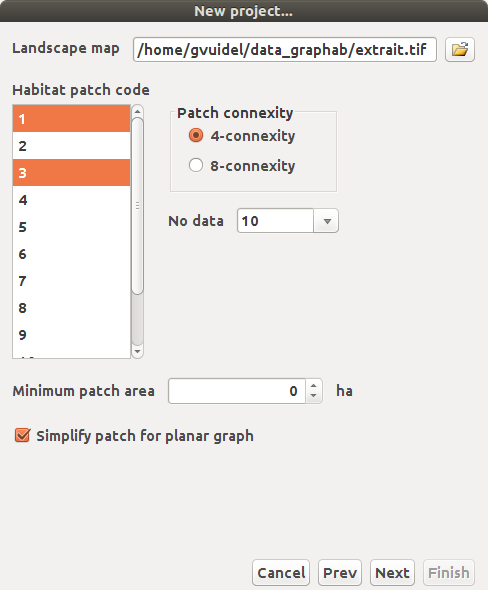
\includegraphics[scale=0.5]{img/manual-en_img3.png}
\end{figure}

If the raster format is *.tif without a Geotiff extension, the file must be associated with a world file for geolocation (*.tfw) structured as follows:

\begin{table}[H]

\begin{tabular}{|m{3.552cm}|m{7.0800004cm}}
\hhline{-~}
Example &
\\\hhline{-~}
10.0 & Pixel size in the X-direction\\
0.0 & Rotation about X-axis \\
0.0 & Rotation about Y-axis \\
{}-10.0 & Pixel size in the Y-direction \\
821755.0 & X coordinate of the center of the upper-left pixel\\
2342995.0 & Y coordinate of the center of the upper-left pixel\\\hhline{-~}
\end{tabular}
\end{table}
If the raster format is *.rst, the file must be associated with a georeferencing file (*.rdc) generated by Idrisi software.  

{\bfseries The units of the image coordinate system must be meters. If not, the areal and distance units will be incorrect. The image can be reprojected in a metric projection (UTM, Lambert93) using GIS software.}

No data: pixel value representing the absence of data in the raster
file.

Habitat patch codes: pixel values assigned to the habitat category used to define habitat patches.  
Several values can be selected by using the \verb|Ctrl| key.


Minimum patch area: minimum area in hectares for a habitat patch to become a graph node.  

Patch connexity:
\begin{itemize}
	\item 4-connexity: a habitat patch consists of the central pixel with its four neighbors if they are of the same value;
	\item 8-connexity: a habitat patch consists of the central pixel with its eight neighbors if they are of the same value.
\end{itemize}

Simplify patch for planar graph: checking the box accelerates the creation of a planar graph, simplifying the polygonal boundaries of patches. This simplification process is not deterministic and so creating two planar graphs for one and the same landscape map may result in slightly different polygon edges. Consequently, this box should not to be checked when planar graphs are to be compared. 

\subsection{Creating link sets}
\label{linkset}
The third window is for creating a link set for which several parameters must be selected: topology and link weighting. Creating a link set is the final step in starting a Graphab project. However, users may create new link sets within the same project via the Graphs / Create link set menu.

\begin{figure}[H]
	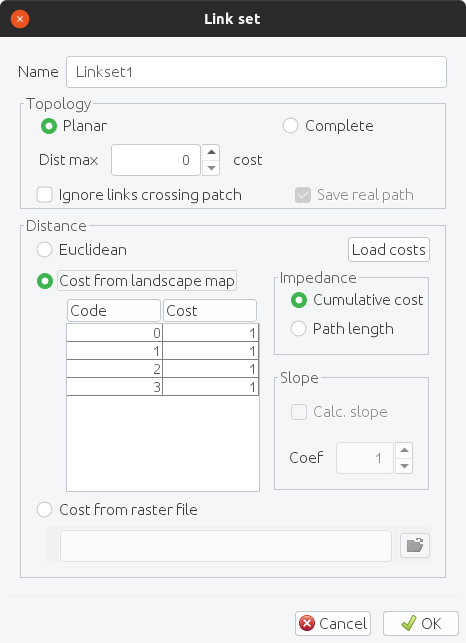
\includegraphics[scale=0.5]{img/manual-en_linkset.png}
\end{figure}


\subsubsection{Link topology}

Two topologies are available: 

\begin{itemize}
	\item planar: only links that form a minimal planar graph are considered. This topology is set up through Voronoi polygons around each habitat patch. These polygons are defined from the edges of patches in Euclidean distance.
	\item complete: all the links between patches are potentially taken into account. 
\end{itemize}

Max distance: this option specifies a threshold distance. Links that exceed this distance are no longer created. This limits the number of links created and so accelerates the creation of the link set. The unit of the distance depends on the type of distance: in meters for the euclidean distance and in cost for the least cost distance.

Ignore links crossing patch: this option means that a link between two patches (A and C in the figure below) which crosses an intermediate patch (B) is not created. It is recommended for calculating the betweenness centrality metric (BC) to take into account how often a patch lies on the shortest path between all pairs of patches in the graph. If the option is unchecked, a link is created between two patches (A and C) crossing an intermediate patch, representing the complete true distance between A and C.

\begin{figure}[H]
	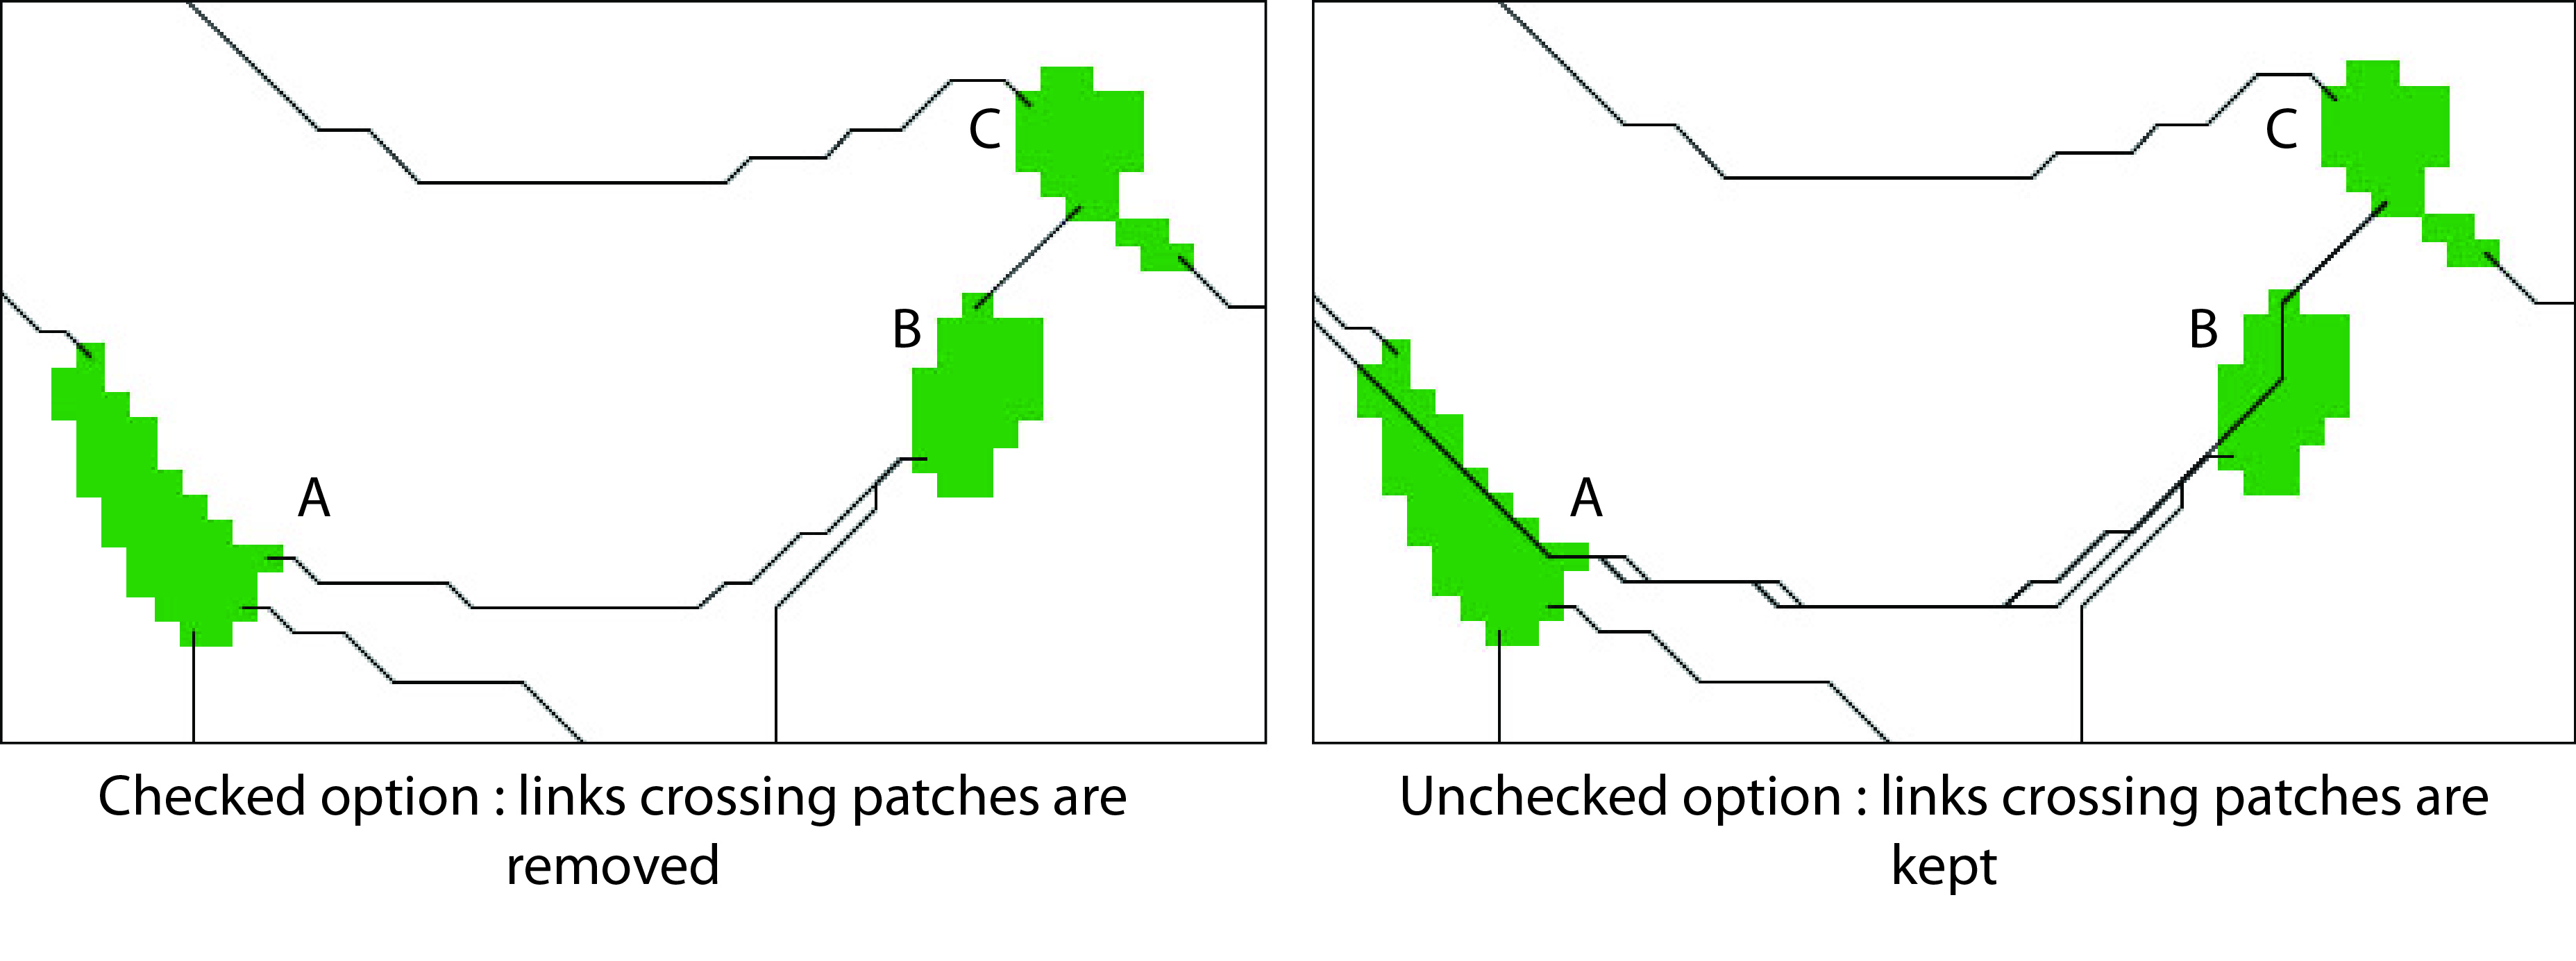
\includegraphics[scale=0.1]{img/manual-en_img5.jpg}
\end{figure}


Save real path: 
\begin{itemize}
	\item checked box: links are saved as paths representing the actual route of the link between two patches.
	\item unchecked box: links are saved in topological form only. In this case, display of links with the realistic view is unavailable. This is recommended for graphs with very many links (e.g. a non-thresholded complete graph) so as to limit the use of memory. Unless paths are saved, intra-patch distances cannot be included in the computation of metrics.
\end{itemize}

\subsubsection{Distance (or link impedance)}

Distances are calculated from edge to edge between patches. Two main types of distance are available: Euclidean distances and least-cost distances.

\begin{itemize}
	\item Euclidean distance: links are defined in Euclidean distances (distance as the crow flies between patches), meaning the matrix is considered to be uniform.
	\item Least-cost distance: links are defined in cost distances. Matrix heterogeneity is taken into account by assigning a resistance value (friction) to each landscape category. The user can activate this option in either of two ways:
	\begin{enumerate}
		\item either by specifying different costs for the landscape map categories in the table,
		\item or from an external raster file (*.tif, *.asc or *.rst) in which each pixel has a resistance value.
	\end{enumerate}
\end{itemize}


The use of least-cost distance provides two types of impedance using the same paths:
\begin{itemize}
	\item cumulative cost: impedance is equal to the sum of the costs of all the pixels along the path,
	\item path length: impedance is equal to the metric length of the path.
\end{itemize}
For each link created, its metric distance and its cost-unit distance are saved and available in “link properties” (see \nameref{properties}). 

Resistance values previously defined can be weighted by slope \cite{2015_monkey}. To compute slope, the DEM should be imported from the menu Data | Set DEM raster. 

The parameter coef ($c$) can adjust the importance of the slope ($p$) weighting. For a given pixel, the resulting resistance value ($r_{final}$) is computed given the formula:  

$$r_{final} = r * (1 + c.p)$$

with the slope $p=\frac{h}{l}$ ratio of the height ($h$) and the length ($l$).\\ 
$p=0$ if the slope is flat, $p=1$ for a slope of 100\% ($h=l$).

When $c=1$ the resistance value is doubled for a slope of 100\%.\\
When $c=10$ the resistance value is doubled for a slope of 10\%.

\section{Graphs}

\subsection{Creating graphs}

A Graphab project may entail the creation of several graphs. Each graph is created from a given link set: either the link set defined in the initial project, or a new link set defined from the Graph / Create link set menu.

Graphs are created from the Graph / Create graph menu. 

\begin{figure}[H]
	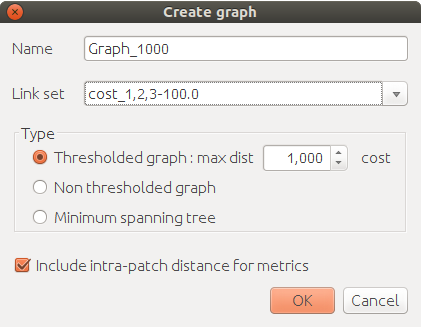
\includegraphics[scale=0.5]{img/manual-en_graph.png}
\end{figure}
	
First, the new graph must be named.

The user must select one of the link sets created previously (cf. \nameref{linkset}) and then select the type of pruning:
\begin{itemize}
	\item None: all links between patches are validated, regardless of length.
	\item Maximum distance: the selected links are less than or equal to the selected maximum distance.	
	\item Minimum spanning tree: graph connecting all the patches in which the total weight of links is minimal.
\end{itemize}

“Include intra-patch distances for metrics” option: if the box is checked, the computation of metrics includes the distances between and across patches (recommended). If the box is unchecked, only the distances between (but not across) patches are taken into account.

For a pruned graph with maximum distance, the unit of the distance depends on the type of distance used in creating the link set. If the link set is created using Euclidean distances, the maximum distance is in meters. If the link set is created using cost distances and the impedance is cumulative cost, the maximum distance is given as a cumulative cost. The unit of the distance (cost or meter) is shown just after the "max dist" field.

\begin{figure}[H]
	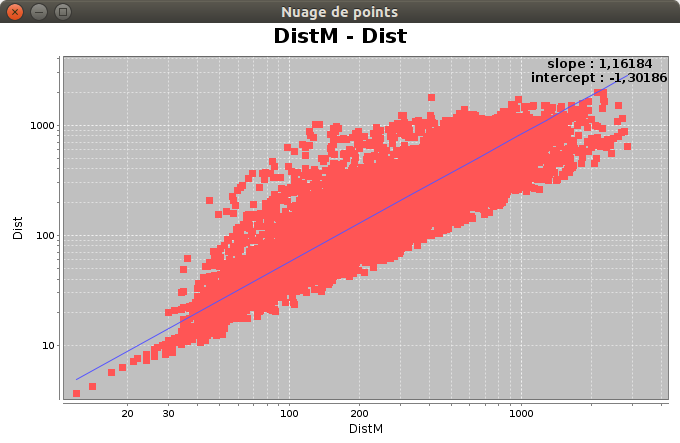
\includegraphics[scale=0.5]{img/manual-fr_img7.png}
\end{figure}

An approximation of the distance metric (DistM) expressed as a cumulative cost (Dist) can be obtained by displaying the double log plot of the link set and using the equation below to perform the conversion:

$$Dist = e^{intercept + slope . log(DistM)}$$

The estimation can be performed directly in Graphab from the menu "Dist. conversion" available by right-clicking on a link set name.

To perform a multiscale analysis, it is often necessary to create a series of graphs in which increasing maximum distances are defined. Users can create this series manually. But if the objective is to analyze the behavior of a metric according to the maximum distance, the Metrics / Batch graphs menu can be used (see \nameref{batch_graph}).


\subsection{Graph clustering}

Graphab implements a clustering algorithm that maximises the modularity index \cite{Newman2006}. Modularity is a measure of the quality of the clustering of the graph nodes. The underlying principle is that a good clustering involves a large number of links within groups and a small number of inter-group links. The algorithm used is based on the greedy algorithm, followed by a local optimization \cite{Brandes2008}.

Modularity is calculated with a weight($w_{ij}$) defined for each link of the graph:
$$w_{ij} = (a_i a_j)^\beta e^{-\alpha d_{ij}}$$
The two parameters $\beta$ et $\alpha$ are used to define respectively the importance of the patch capacity ($a_i a_j$) and the importance of the distance ($d_{ij}$) for the weight of the link $w_{ij}$. If $\alpha = \beta = 0$, then the weights are identical: $w_{ij} = 1$.  

The graph clustering is available by right-clicking on the name of the graph. In the first window, the user defines the parameters $\alpha$ et $\beta$. The parameter $\alpha$ is not defined directly, it is determined from two other parameters: a distance $d$ and a probability $p$ (cf. \nameref{param_weight}). To define $\alpha$ to 0, $p$ must be equal to 1.\\
The right part of the window allows to select which clustering to keep in memory. By default, all clustering are kept in memory to display them after. These settings are useful to avoid memory overflow with large graphs (more than 5,000 nodes). In this case, graphab can keep only the best clustering (ie. with the best modularity) or keep all clustering in a given size interval between 1 and the number of nodes.

\begin{figure}[H]
	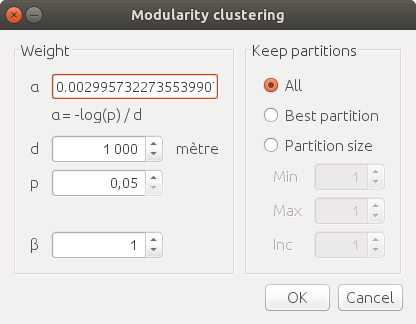
\includegraphics[scale=0.36]{img/manual-en_clustering.png} 
\end{figure}

After validating this window, the calculation starts until a clustering maximizing modularity is obtained. The result is displayed as a new layer of the graph. Two other windows complete this result.

\begin{figure}[H]
	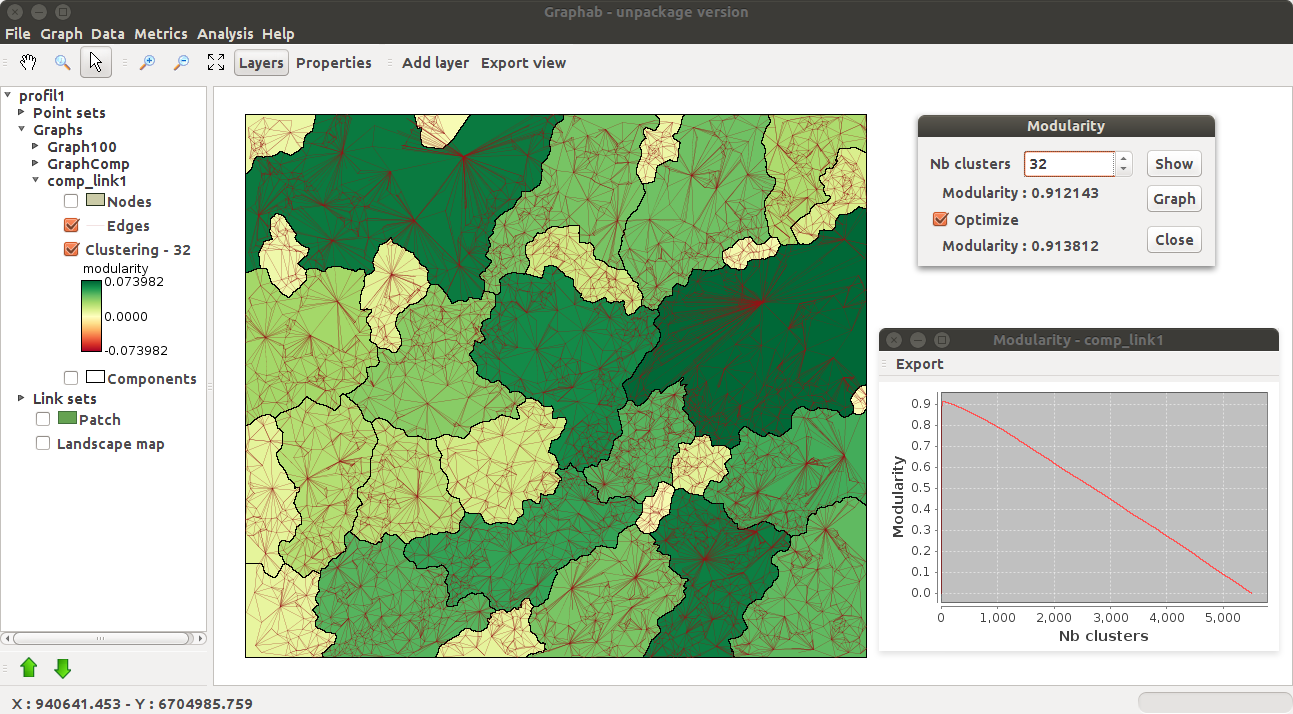
\includegraphics[scale=0.36]{img/manual-en_cluster.png} 
\end{figure}

The new layer shows the elements of the spatial partition as polygons. Since a given element corresponds to a set of patches, it is represented by a polygon resulting from the aggregation of the Voronoï’s polygons of all patches of the cluster. The modularity value is used to assign a color to the polygon. The overall modularity is the sum of the modularity values of all clusters. 

In a first window, a graph shows how modularity varies according to the number of clusters. In the previous figure, the maximal modularity is reached with a small number of clusters.

The second window displays the number of clusters that maximizes modularity and the value of modularity.
Several functions are available from this window:\\
{}- the number of clusters can be changed to show sub-optimal partitions. The result may be visualized by clicking on the button "Show". The new layer of partition is added to the graph.\\
{}- the button "Graph" allows you to create a new graph including only the intra-cluster links.\\
{}- the checkbox "Optimization" achieves a local optimization of the clustering after the use of the greedy algorithm, that significantly improves the modularity value. This option is enabled by default.


\section{Corridors}

Graphab allows to calculate the corridors representing, for a given maximum distance $d_{max}$, the area that can be traversed between 2 patches habitat \textit{ie.} the area representing the set of possible paths connecting 2 patches and having a distance less than the distance $d_{max}$.

Corridors can be calculated only from a linkset that has been defined from costs. To use this feature, just right click on a linkset and click on "Corridor".
The maximum cost distance $d_{max}$ must be entered before launching the calculation.	

\begin{figure}[H]
	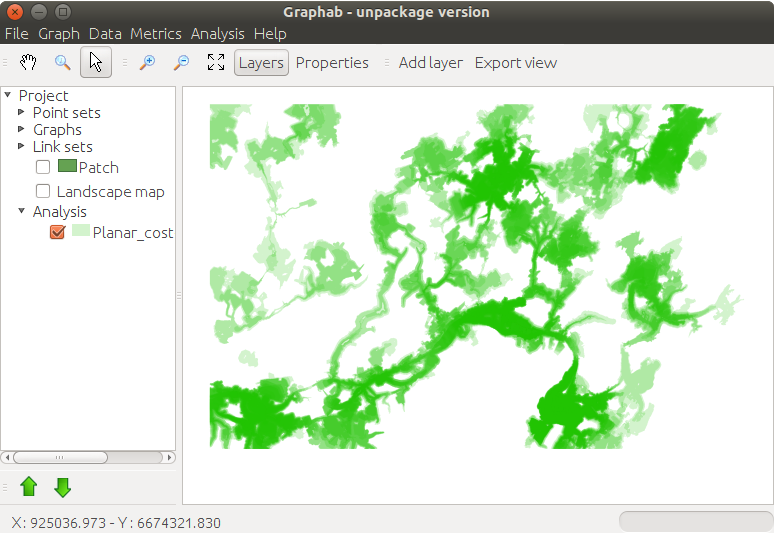
\includegraphics[scale=0.5]{img/manual-en_corridor.png} 
\end{figure}

The result is displayed in a new vector or raster layer depending on the selected output. In vector output, the layer contains for each link of the selected linkset a polygon representing its corridor. Links with a distance greater than $d_{max}$ will have no corridor.
In raster output, each pixel contains the number of corridors passing through it.

For vector layer, the default view uses transparency to show corridor overlays.


\section{Patch capacity}

The capacity of a patch reflects its intrinsic quality as an indicator of its demographic potential. A patch with a high capacity can accommodate a large population and vice versa. Capacity is included directly in the calculation of some area connectivity metrics and weighted connectivity metrics (see \nameref{metric_fam}).

When the project is first created the patch capacity is equal by default to the patch area in m². However, users may replace area by any other quality indicator. In some cases, species presence is related not to patch size but to the area of other types of land cover around the patch. For example, the presence of amphibians in a breeding pond does not depend on the pond size but on the amount of terrestrial habitat
surrounding the pond.

The Data / Set patch capacity menu can be used to modify the capacity of all patches by two methods.

\subsection{Capacity as a function of the neighborhood}

The first method can be used to define patch capacity as a function of the neighborhood composition and to calculate it directly from Graphab. 

\begin{figure}[H]
	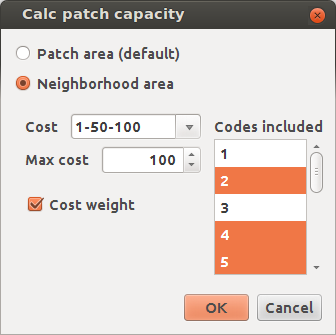
\includegraphics[scale=0.5]{img/manual-en_img8.png}
\end{figure}

Users must define three parameters: type of distance, maximum distance, landscape categories.

Cost: This is the spatial metric (Euclidean or cost distance) corresponding to one link set available in the project. The use of costs in this procedure amounts to defining an anisotropic neighborhood around patches which may differ greatly from a buffer function. For consistency, it is recommended to use the same type of distance as was
used in creating the links of the graph. For a link set created with Euclidean distance, the user must select “all costs = 1”.

Max cost: Like the graph maximum distance, the unit of this maximum distance depends on the type of distance used in creating the link set (Euclidean or cost distance).

Codes included: the user may select one or more landscape categories, other than the habitat category, to be included in calculating capacity.

The “cost weight” option introduces a weighting with distance to the patch through a negative exponential function. In this way, the areas selected have greater weight if they are close to the patch and vice versa.

The capacity values calculated replace the patch area for all subsequent computations. But users can return to the initial parameter via the Data / Set patch capacity menu and by selecting "Patch area".

\subsection{Capacity defined from external data}

The second method is for importing a data table (*.csv) describing all the patches of the project and containing capacity values defined in advance by the user. The patch identifiers in the table must be the same as the patch identifiers in the Graphab project.

The capacity values in the imported table replace patch area values for all subsequent computations after importing. But users can restore the initial parameter via the Data / Set patch capacity menu and by selecting “Patch area”.

\begin{figure}[H]
	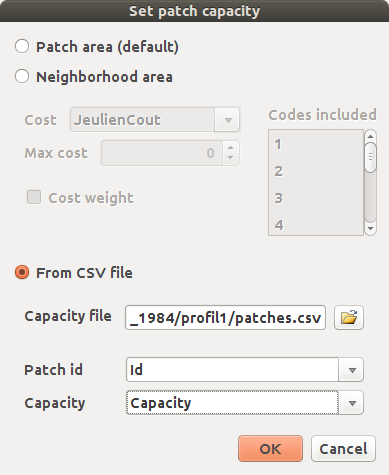
\includegraphics[scale=0.5]{img/manual-en_img9.png}
\end{figure}

\subsection{Patch removing}

After setting patches capacity, it can be useful to remove patches whose capacity is too low. The entry "Remove patches" from the Data menu, lets you create a new project identical to the current project and remove patches with a capacity below a given threshold.

After entering the required minimum capacity, the new project is created in a subdirectory of the current project and directly loaded.


\section{Calculating connectivity metrics}

\subsection{Metrics family and computing level}
\label{metric_fam}
Each graph in a project can be used to compute different connectivity metrics. The details of how they are computed and references are listed in the Annex. Computations are made at several levels corresponding to major sections in the Metrics menu (table \ref{metric_level}):
\begin{itemize}
	\item Metrics /Global metrics: describe the entire graph.
	\item Metrics /Component metrics: describe connectivity within each component (or sub-graph).
	\item Metrics /Local metrics: describe the connectivity of each graph element (node or link).
	\item Metrics /Delta metrics: also describe each graph element, but using a specific computing method. Using the removal method (remove nodes or remove links), the relative importance of each graph element is assessed by computing the rate of variation in the global metric induced by each removal. The result of a delta-metric is at a local level but by reference to the global level.
\end{itemize}

After selecting one of these four computing methods, three families of
metrics are available in the new window: 
\begin{itemize}
	\item weighted metrics are based on criteria of distance and patch capacity. They have to adjusted to suit the reference species. These metrics involve computing paths in a graph via Dijkstra{\textquotesingle}s algorithm. After selecting one of these metrics, the user must specify the desired adjustment.
	\item area metrics are based primarily on the area criterion. If capacity corresponds to a criterion other than patch area, these metrics can be computed and they are expressed in the unit of the criterion used.
	\item topological metrics are derived from graph theory and they do not require adjustment.
\end{itemize}

Whichever the selected level, the user must first specify the graph on which the calculation will be made and then select the connectivity metric.

\begin{table}[H]
	\begin{tabular}{|c|l|l|c|c|c|c|}
		\hline
		Family & Connectivity metrics & Code & \multicolumn{3}{m{3.6cm}|}{\centering Computing level} & Delta metrics\\
		\hhline{~~~---~}
		& & & Global & Comp. & Local &\\
		\hline
		Weighted
		& \nameref{metric_F} & F & × & × & × &\\
		\hhline{~------}
		& \nameref{metric_EC} & EC & × & × &  & ×\\
		\hhline{~------}
		& \nameref{metric_PC} & PC & × & × &  & ×\\
		\hhline{~------}
		& \nameref{metric_IF}  & IF &  &  & × &\\
		\hhline{~------}
		& \nameref{metric_dPC} & dPC &  &  &  & ×\\
		\hhline{~------} 
		& \nameref{metric_BC} & BC &  &  & × & \\
		\hhline{~------}
		& \nameref{metric_IIC} & IIC & × & × &  & × \\
		\hhline{~------}	
		& \nameref{metric_CF} & CF &  &  & × & \\
		\hline
		Area
		& \nameref{metric_MSC} & MSC & × &  &  & \\
		\hhline{~------}
		& \nameref{metric_SLC} & SLC & × &  &  & \\
		\hhline{~------}
		& \nameref{metric_CCP} & CCP & × &  &  & \\
		\hhline{~------}
		& \nameref{metric_ECS} & ECS & × &  &  & \\
		\hline
		Topological 
		& \nameref{metric_Dg} & Dg &  &  & × & \\
		\hhline{~------}
		& \nameref{metric_CC}  & CC &  &  & × & \\
		\hhline{~------}
		& \nameref{metric_CCe} & CCe &  &  & × & \\
		\hhline{~------}
		& \nameref{metric_Ec} & Ec &  &  & × & \\
		\hhline{~------}
		& \nameref{metric_CCor} & CCor &  &  & × & \\
		\hhline{~------}
		& \nameref{metric_NC} & NC & × &  &  & \\
		\hhline{~------}
		& \nameref{metric_GD} & GD & × & × &  & ×\\
		\hhline{~------}
		& \nameref{metric_H} & H & × & × &  & ×\\
		\hhline{~------}
		& \nameref{metric_W} & W & × &  &  & \\
		\hline
	\end{tabular}
	\caption{Connectivity metrics and computing level}
	\label{metric_level}
\end{table}

\subsection{Parameters of weighted metrics}
\label{param_weight}

\begin{figure}[H]
	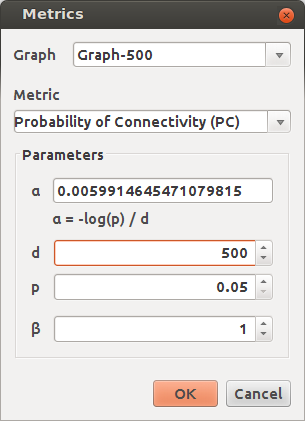
\includegraphics[scale=0.5]{img/manual-en_img10.png}
\end{figure}


\subsubsection{Alpha parameter}

Several metrics include a weighting in their calculation which converts the distance between patches into the probability of movement. These metrics are F, IF, PC, EC, BC... The weighting is based on an exponential function:
\begin{equation*}
p={e}^{-\mathit{\alpha d}}
\end{equation*}
where $p$ is the probability of movement between two patches, $d$ the distance between these patches, and $\alpha$ a parameter defining the rate of decline in probability as distance increases. As it is not easy to determine the value of the $\alpha$ parameter, Graphab calculates it from the other two parameters. Users must specify the distance corresponding to a certain value of probability, e.g.:
\begin{itemize}
	\item the maximum dispersal distance of species corresponding to a small value of $p$ (0.05 or 0.01).
	\item the average dispersal distance of species corresponding to a median value of $p$ (0.5).
\end{itemize}

The value of $\alpha$ is automatically obtained from the formula:
\begin{equation*}
\alpha =-\log \left(p\right)/{d}
\end{equation*}


\subsubsection{Beta parameter}

The metrics F, IF, CF, and BC are controlled by the $\beta$ parameter. This parameter is the exponent applied to patch capacity. It adjusts the relative balance between the weight of distances and the weight of patch capacity in the weighting of metrics. Taking the example of the metric F in local computation, whose generic form is:
\begin{equation*}
F=\sum {{a}^{\beta }}{e}^{-\mathit{\alpha d}}
\end{equation*}

\begin{itemize}
	\item a value of $\beta =0$ means that the patch capacity plays no part in the weighting.
	\item a value of $\beta =1$ means that the patch capacity acts linearly in the weighting.
	\item a value of $\beta =2$ means that the patch capacity is squared in the weighting.
	\item a value of $\beta =0.5$ means that the square root of the patch capacity features in the weighting.
	\item a value of $\beta =-1$ means that the patch capacity acts in an inversely proportional way in the weighting.	
\end{itemize}

In addition to these few examples, any weighting values are possible.

\subsection{Calculating batch metrics}

Every metric compatible with the global level can be calculated following the variation of the scale of distances. This variation may concern either graph pruning (\ref{batch_graph}), or metric adjustment (\ref{batch_metric}). The type of distance used depends on the type of distance used in creating the link set (Euclidean, least-cost distance, or least-cost path).

\subsubsection{Batch graph}
\label{batch_graph}
The Metrics / Batch graph menu allows a series of pruned graphs to be created from a given link set and a metric to be calculated for each graph at global level. The maximum distance of successive graphs are increasingly defined in either of two ways:
\begin{itemize}
	\item distance: a fixed increment of distance is defined between successive graphs. The metric values are therefore calculated inregular intervals of  distance.
	\item number of links: a fixed number of links is defined between successive graphs. This number of links is automatically converted into distance used to prune the graph. These distances may be unevenly spread.
\end{itemize}

\begin{figure}[H]
	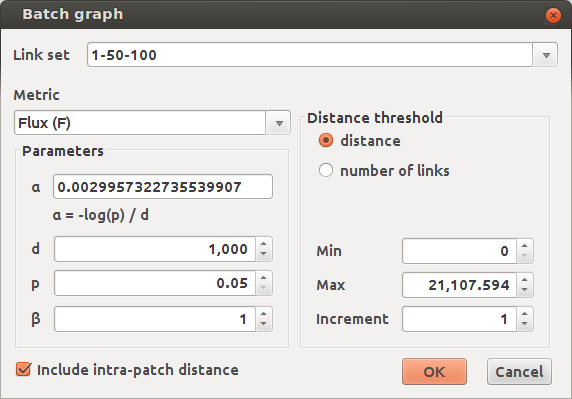
\includegraphics[scale=0.5]{img/manual-en_img11.png}
\end{figure}

Graphs are defined following three criteria selected by users:
\begin{itemize}
	\item min: smallest distance used for the first graph in the series. By default, this minimum is 0, corresponding to the total absence of links.
	\item max: maximum distance used for the final graph in the series. By default, this maximum corresponds to the maximum distance or to the link number of the selected link set.
	\item increment: distance value added between each new graph.
\end{itemize}

Once the calculation is completed, the software opens a new window displaying the curve of the selected metric versus the maximum distance. The values of this curve can be saved with the “Export” button by selecting text format.

\subsubsection{Batch parameter}
\label{batch_metric}
The Metrics / Batch parameter menu is used to calculate a series of metrics from a given graph. This procedure applies to the weighted metrics only. It is divided into two entries: local metrics or global metrics.

\textbf{Batch parameter for local metrics}

A local weighted metric is calculated in series according to the variation of one of its parameters. The user must select the graph, the metric, and the parameter to be varied. The variation of computation is defined by:
\begin{itemize}
	\item min: minimum value of the parameter,
	\item max: maximum value of the parameter,
	\item increment: interval value between two metric computations.
\end{itemize}

Once the calculation is completed, the patches (and in some cases the links) of the graph are characterized by a series of additional metrics.

\textbf{Batch parameter for global metrics}

For a given graph, a global weighted metric is calculated in series according to the variation of one of its parameters. As previously, this variation is defined between a minimum value (min), a maximum value (max), and with an interval (increment). 

The procedure ends with the opening of a new window displaying the curve of the selected metric versus the parameter. 

Table \ref{metric_poss} summarizes possible metrics calculations.

\begin{table}[H]
\begin{tabular}{|c|p{5cm}|l|>{\centering\arraybackslash}m{1.5cm}|>{\centering\arraybackslash}m{1.5cm}|>{\centering\arraybackslash}m{0.8cm}|>{\centering\arraybackslash}m{0.8cm}|>{\centering\arraybackslash}m{1cm}|>{\centering\arraybackslash}m{1cm}|}
\hline
Family & Connectivity metrics & Code & Patch capacity & Intra-patch distance  & \multicolumn{2}{m{1.8cm}|}{\centering Parameters} & Batch graph & Batch param\\
\hhline{~~~~~--~~}
 & & & & & $\alpha$ & $\beta$ & & \\
\hline
Weighted
 & Flux & F & × & × & × & × & × & ×\\
 & Equivalent Connectivity & EC & × & × & × & & × & ×\\
 & Probability of connectivity & PC & × & × & × & & × & ×\\
 & Interaction Flux  & IF & × & × & × & × &  & ×\\
 & Fractions of delta Probability of connectivity & dPC & × & × & × &  &  &\\
 & Betweenness centrality index & BC & × & × & × & × &  &×\\
 & Integral index of connectivity & IIC & × &  &  &  & × & \\
 & Current flow & CF & × &  &  & × &  & ×\\
\hline
Area
 & Mean size of the components & MSC & × &  &  &  & × & \\
 & Size of the largest component & SLC & × &  &  &  & × & \\
 & Class coincidence probability & CCP & × &  &  &  & × & \\
 & Expected cluster size & ECS & × &  &  &  & × & \\
\hline
Topological
 & Node Degree & Dg &  &  &  &  &  & \\
 & Clustering coefficient  & CC &  &  &  &  &  & \\
 & Closeness centrality & CCe &   & x &  &  &  & \\
 & Eccentricity & Ec &  & x &  &  &  & \\
 & Connectivity correlation & CCor &  &  &  &  &  & \\
 & Number of components & NC &  &  &  &  & × & \\
 & Graph diameter & GD &  & × &  &  & × & \\
 & Harary Index & H &  &  &  &  & × & \\
 & Wilks' Lambda & W &  &  &  &  & × & \\
\hline
\end{tabular}
\caption{Possible connectivity metrics calculations}
\label{metric_poss}
\end{table}

\subsection{Interpolating metrics}

The Analysis / Metric interpolation menu is used to create raster layers from local metrics calculated at patch level. This transformation is based on a specific spatial interpolation which assigns connectivity values of patches to each cell of a grid, using a decreasing weighting function from the patch edge (weight of 1). Overall, the farther cells are away from the graph, the lower their connectivity values. 

The weighting is a negative exponential function as $p={e}^{-\mathit{\alpha d}}$ for which the user selects a distance ($d$) corresponding to a certain probability ($p$) and the software deduces the value of the $\alpha$ parameter. In theory, this adjustment must be consistent with the choice of reference graph or of any weighted metrics, using the same value of $d$. 

The Multi connection option allows several patches to be included in the calculation of metrics at the point level. The calculation is based on a sum or a weighted mean of values of all patches in the vicinity of the points, up to the specified Maximum distance. 

The distance used in these calculations depends on the reference graph. If it is based on least-cost distance, the spatial interpolation uses the same distance and not Euclidean distance.

The metric interpolation is used automatically in calculating species distribution models; see \nameref{sdm}.


\section{Patch addition}

The function "Add patches" is available in the menu "Analyses". It is used to test a set of locations to create new habitat patches according to the connectivity gain they provide. Graphab calculates first the selected global connectivity metric, then it adds virtually a patch and the links between this patch and existing patches (only if their distance is less than the maximum distance of the graph in the case of a pruned graph) and calculates the global metric again. Once all locations are tested, the software validates the one for which patch addition produces the biggest increase in the metric value. The process is repeated until the desired number of additional patches is reached by including elements already added at each step.

\begin{figure}[H]
	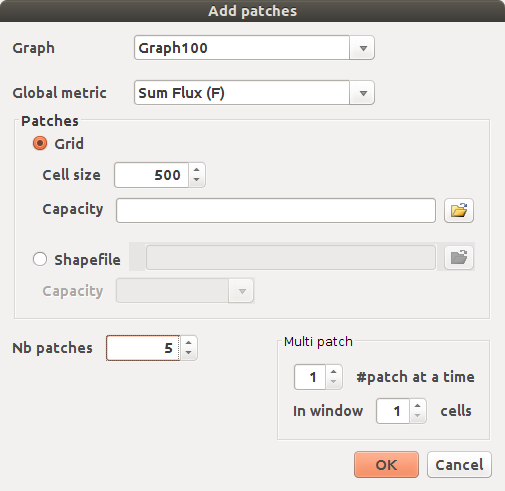
\includegraphics[scale=0.5]{img/manual-en_addpatch.png} 
\end{figure}

Several parameters must be defined:
\begin{itemize}
	\item Graph: the graph used for computing the connectivity metric and adding new patches. The underlying link set must be in complete topology.
	\item Global metric: the global metric to maximize and his settings (Parameters button)
	\item Nb Patches: number of patches (which become new nodes of the graph) to be added.
\end{itemize}

The definition of the patch set to test can be done in two ways:
\begin{itemize}
	\item by automatically applying a grid of a given resolution (field "cell size" to define). In this case, Graphab tests each centroid of the cells by adding a virtual new patch. By default, all centroids have the same capacity value (=1). Nevertheless, it is possible to import a raster layer in which each pixel of the lansdcape matrix has its own capacity value,
	\item by importing a shapefile of points or polygons. In this case, the user must indicate which column of the attribute table contains the patch capacity.
\end{itemize}

Multi-patches option : this option can be used to test the addition of several patches simultaneously. The additionnal patches are searched in a neighbourhood window of x cells (parameter to define) around the first patch.

At the end of the calculation, a folder named "addpatch\_nX-GraphX\_..." is created and saved in the project directory. It contains:
\begin{itemize}
	\item a shapefile containing the added nodes. The attribute table indicates the step at which each node was validated and the corresponding value of the  global metric,
	\item two shapefiles containing all the links of the graph, including those connecting the new nodes in topological form ("topo\_links\_graphXXX") or in realistic form ("links\_graphXX"),
	\item a raster "landuse.tif" containing the modified land use,
	\item a folder named "detail" containing the shapefile of the tested locations and the corresponding value of the global metric for each step. 
\end{itemize}

References : 
\cite{2015_addpatch_rainette, 2014_LUP}



\section{Meta-patch}

From the Graph menu, the "Create metapatch project" entry creates a new project where the nodes of the graph correspond to sets of interconnected patches. This feature allows to better take into account the nested scales of ecological processes, especially the functional definition of a habitat patch that is dependent on the scale considered.

\begin{figure}[H]
	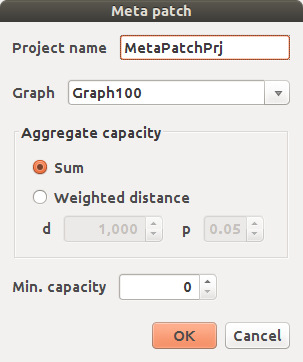
\includegraphics[scale=0.5]{img/manual-en_metapatch.png} 
\end{figure}

To use this feature, it is necessary to create an initial project and a graph pruned at the desired distance (eg daily distance). Each component of this pruned graph correspond to a meta-patch. It is therefore constituted by all interconnected patches.

By default, the metapatch capacity is defined as the sum of the capacity of the patches composing the metapatch. The other option, "Weighted distance", is used to reflect the removal between patches. For this option, you must define the parameter $\alpha$ by giving a distance $d$ and an associated probability $p$ (see \nameref{param_weight}). The resulting capacity ($C$) of a metapatch is:

$$C = \frac{1}{n}\sum_{i}^n\sum_{j}^n c_j e^{-\alpha d_{ij}}$$ 

The "Min. capacity" option keeps only the metapatch that have a capacity greater than or equal to the given capacity.

The new project is saved in a subdirectory of the original project and is automatically loaded at the end of the process.

Reference : \cite{2015_monkey}


\section{Connecting graphs and point data}

The main part of the software is for graph construction and computation of connectivity metrics. But it is often useful to connect these elements with external data. Graphab allows graph data to interact with a points data set.

\subsection{Importing points sets}

Point data can be imported via the Data / Import point set menu. These data may contain several attributes but only binary attributes (presence/absence) are taken into account in certain procedures (see \nameref{sdm}).

\begin{figure}[H]
	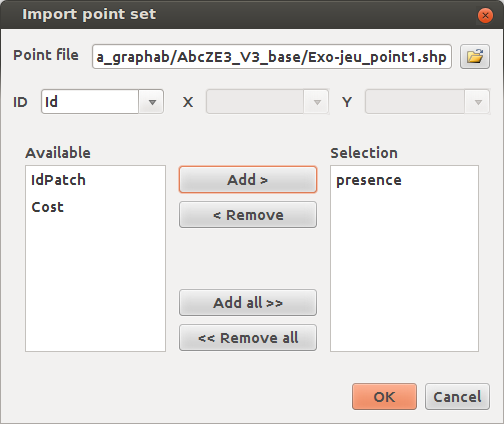
\includegraphics[scale=0.5]{img/manual-en_img12.png}
\end{figure}

The imported file may be either in shapefile format (*.shp), or in table format (*.csv). For files in table format, the user must specify the columns corresponding to identifiers and to the XY coordinates of points in the table. The attributes to be considered must be selected from the list of attributes available.

If point data do not contain an absence attribute, they cannot be used in species distribution models. If the user wants to set up a species distribution model, a set of pseudo-absence points can be generated by the Data / Generate random point menu.

\subsection{Inter-point distance matrix}

Point data imported to Graphab can be used to calculate the inter-point distance matrix by right-clicking on the name of the point data and selecting "Distance matrix".

\begin{figure}[H]
	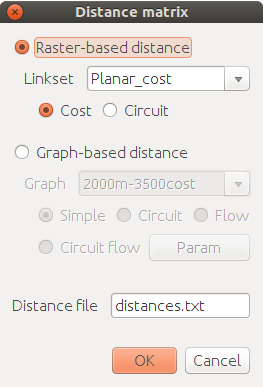
\includegraphics[scale=0.5]{img/manual-en_point_matrix.png} 
\end{figure}

Two types of distance are available: raster-based distance and graph-based distance.

\subsubsection{Raster-based distance}

In raster mode, the distances are calculated based on the selected link set. This link set can not be euclidean.

According to the selected link set, the resulting distances may be the cumulative cost  distance or the length of the least cost path. In both cases, the calculation includes  costs assigned to the landscape map categories, as defined when creating the link set. The result is a distance matrix which is independent of the graph; this matrix corresponds to the calculation provided by the Geographicinformation Systems. 

The Circuit option allows to calculate another distance between each point by calculating the resistance distance, i.e. the total resistance of an electrical circuit of resistors instead of calculating the shortest path. This method considers all possible paths and not only the shortest one (cf. \cite{McRae2008}).


\subsubsection{Graph-based distance}
In graph mode, the distances are calculated based on the selected graph. This graph must be based on the link set used for point set import.
\begin{itemize}
	\item Least cost : calculates distances according to the shortest path in the selected graph. The type of distance is the same as that used in creating the link set of the selected graph. At both ends of a given path, the calculation includes the distance between each point and the nearest patch. Depending on the choice made when creating the graph, the calculation may or may not include intra-patch distances.
	\item Circuit : calculates the resistance distance between the closest patch of each point. The graph is seen as an electrical circuit where each link of the graph represents a resistor. This option considers all possible paths, not just the shortest one.
\end{itemize}

\subsection{Generating random points}

The Data / Generate random points menu can be used to generate a set of pseudo-absence points based on a set of presence points.

\begin{figure}[H]
	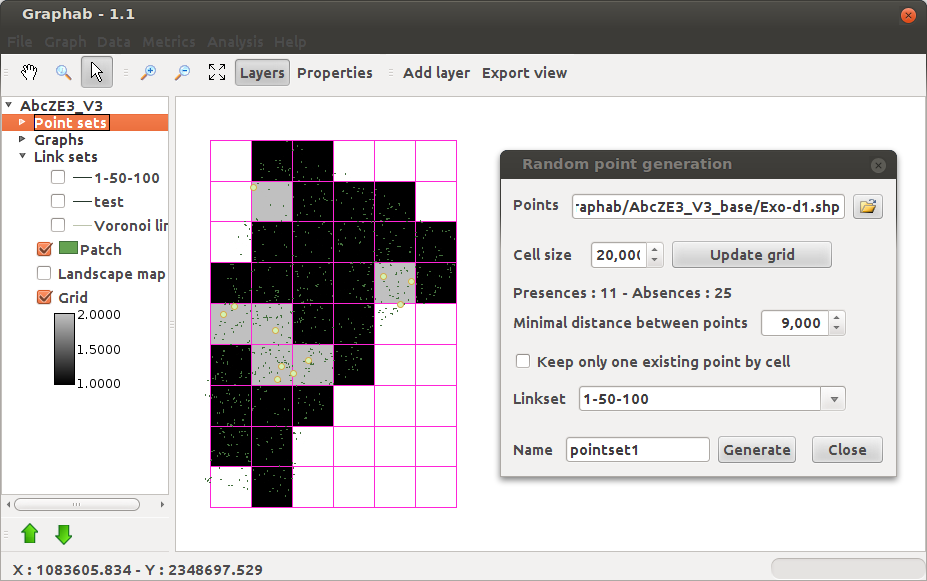
\includegraphics[scale=0.5]{img/manual-en_img13.png}
\end{figure}
 

The user must load a file of presence points and specify the name of the set of presence/pseudo-absence points to be created.

Several parameters must be defined to randomly sample absence points:
\begin{itemize}
	\item Cell size of the grid (in meters) to define the size of cells from which absence points will be potentially sampled. The “update grid” button can be used to display the grid according to the selected cell size. 
	\item Minimum distance between points: this function reduces the effects of spatial autocorrelation by specifying a minimum distance in meters to be observed between the generated absence points and between these points and presence points.
	\item Type of distance: the unit of the minimum distance between points depends on the type of the distance used in the link set selected.
	\item Keep only one existing point by cell: this option (checked box) retains only one presence point in each cell thereby reducing the effects of spatial autocorrelation.
\end{itemize}

\subsection{Species distribution model}
\label{sdm}
If a set of presence/absence points has been defined, the software can use the connectivity metrics calculated from a graph as predictors in a species distribution model from the Analysis / Species distribution model menu. Such modeling is possible even if points are not located in habitat patches, by means of a spatial extrapolation of the values of metrics. The logistic regression model is a based on minimizing the AIC
criterion.

\begin{figure}[H]
	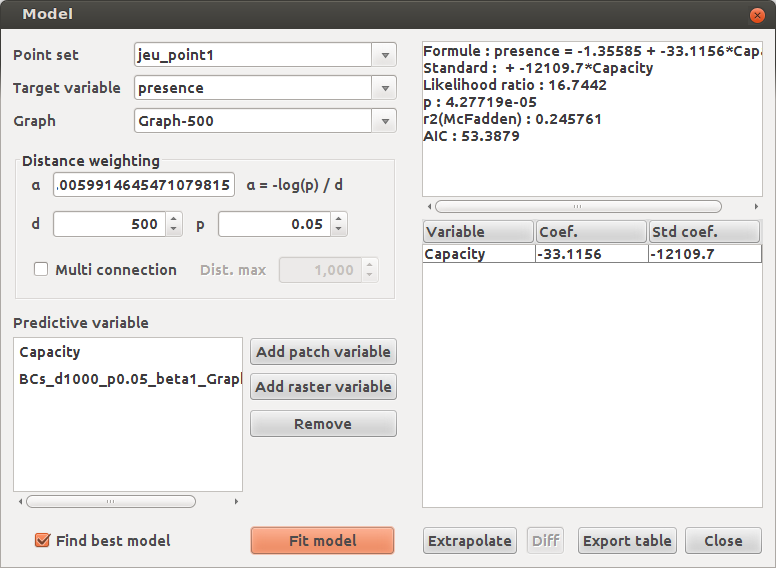
\includegraphics[scale=0.5]{img/manual-en_img14.png}
\end{figure}


First, the user must specify:
\begin{itemize}
	\item the set of point data to use,
	\item the target variable in the predictive model,
	\item the reference graph for the use of connectivity metrics.
\end{itemize}

\subsubsection{Weighting for extrapolating metrics to points}

The values of metrics are calculated for any point by a spatial interpolation. This interpolation is based on values being weighted by a decreasing function from patch edges (weight of 1). The weight decreases as the same negative exponential function as the one used for weighted metrics (see \nameref{param_weight}), the adjustment is therefore
identical. 

The user selects a distance (d) corresponding to a certain probability (p) and the software deduces the value of the $\alpha $ parameter. In principle, this adjustment must be consistent with the choice of reference graph or of any weighted metrics included in the model, using the same value of d.

The Multi connection option allows several patches to be included in calculating metrics at points. Calculation is based on the weighted mean of values of all patches surrounding points, up to the specified Maximum distance.

Details of this weighting are given in \cite{2012_SDM}.

\subsubsection{Estimating the model}

The selection of a graph to perform the model displays all available connectivity metrics among predictive variables.

Metrics from another graph can be added by clicking on the Add patch variable button.

External variables can also be added by clicking on the Add external variable button.

Once the predictor variables have been selected, the Fit model button can be used to calculate the coefficients of the logistic regression. The results are displayed on the right-hand side of the window. The Find best model option tests all possible combinations of variables and selects the one that minimizes the AIC criterion.

\subsubsection{Using the model}

A predictive model which is considered to be valid can be used in several ways.

The Export table button can be used to export a table (*.csv format) with all statistical variables involved in the regression.

The Extrapolate button provides an estimation of the probability of the species presence in all cells of a grid. 


\begin{figure}[H]
	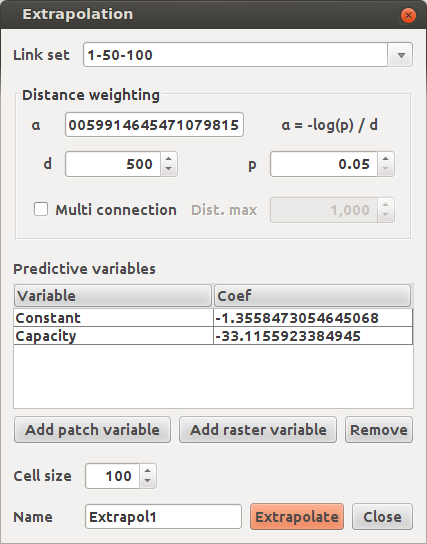
\includegraphics[scale=0.5]{img/manual-en_img15.png}
\end{figure}


In the new window which opens, the user finds the model parameters as described previously. The cell size of the grid (in meters) indicates the level of spatial accuracy of the extrapolation. This parameter has a significant consequence on the computing time required to obtain the result. The result is saved as a raster layer in *.tif format and is displayed in the main window.

\bigskip
References : \cite{2012_SDM, 2012_graphab_EMS, 2013_SDM, 2013_SDM_rainette}

\section{Display}

\subsection{Graph properties}

Properties of a graph are available by right-clicking on the name of the graph. Two ways for viewing graphs are available: 
\begin{itemize}
	\item The topologic view displays a simplified view of the graph in which nodes are represented by dots and links by straight lines between centroids.
	\item The realistic view displays habitat patches according to their actual boundaries and links are represented by least-cost paths between two patches.
\end{itemize}

\begin{figure}[H]
	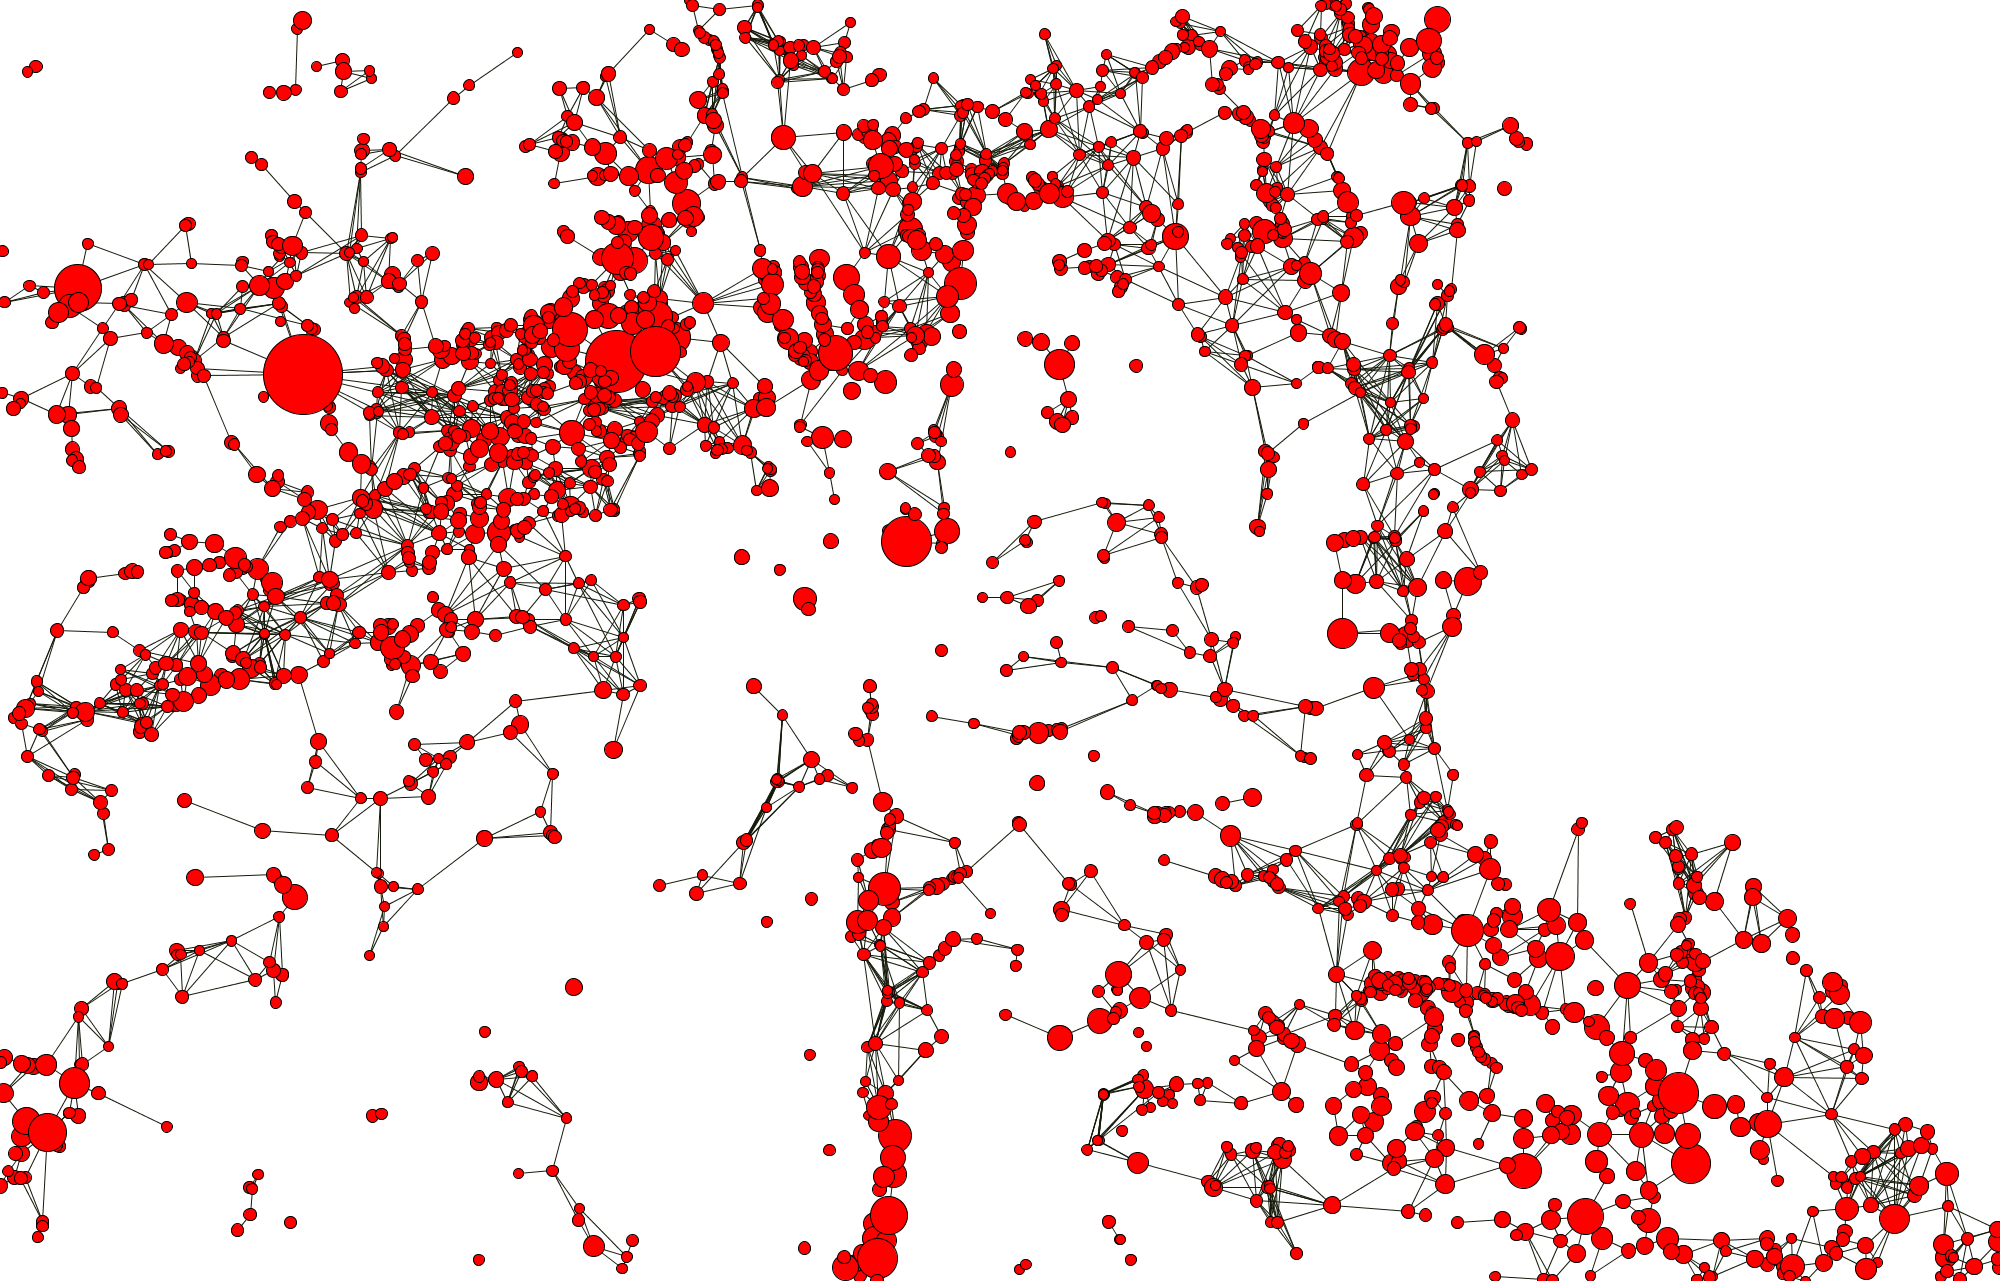
\includegraphics[scale=0.1]{img/manual-en_img16.png}
	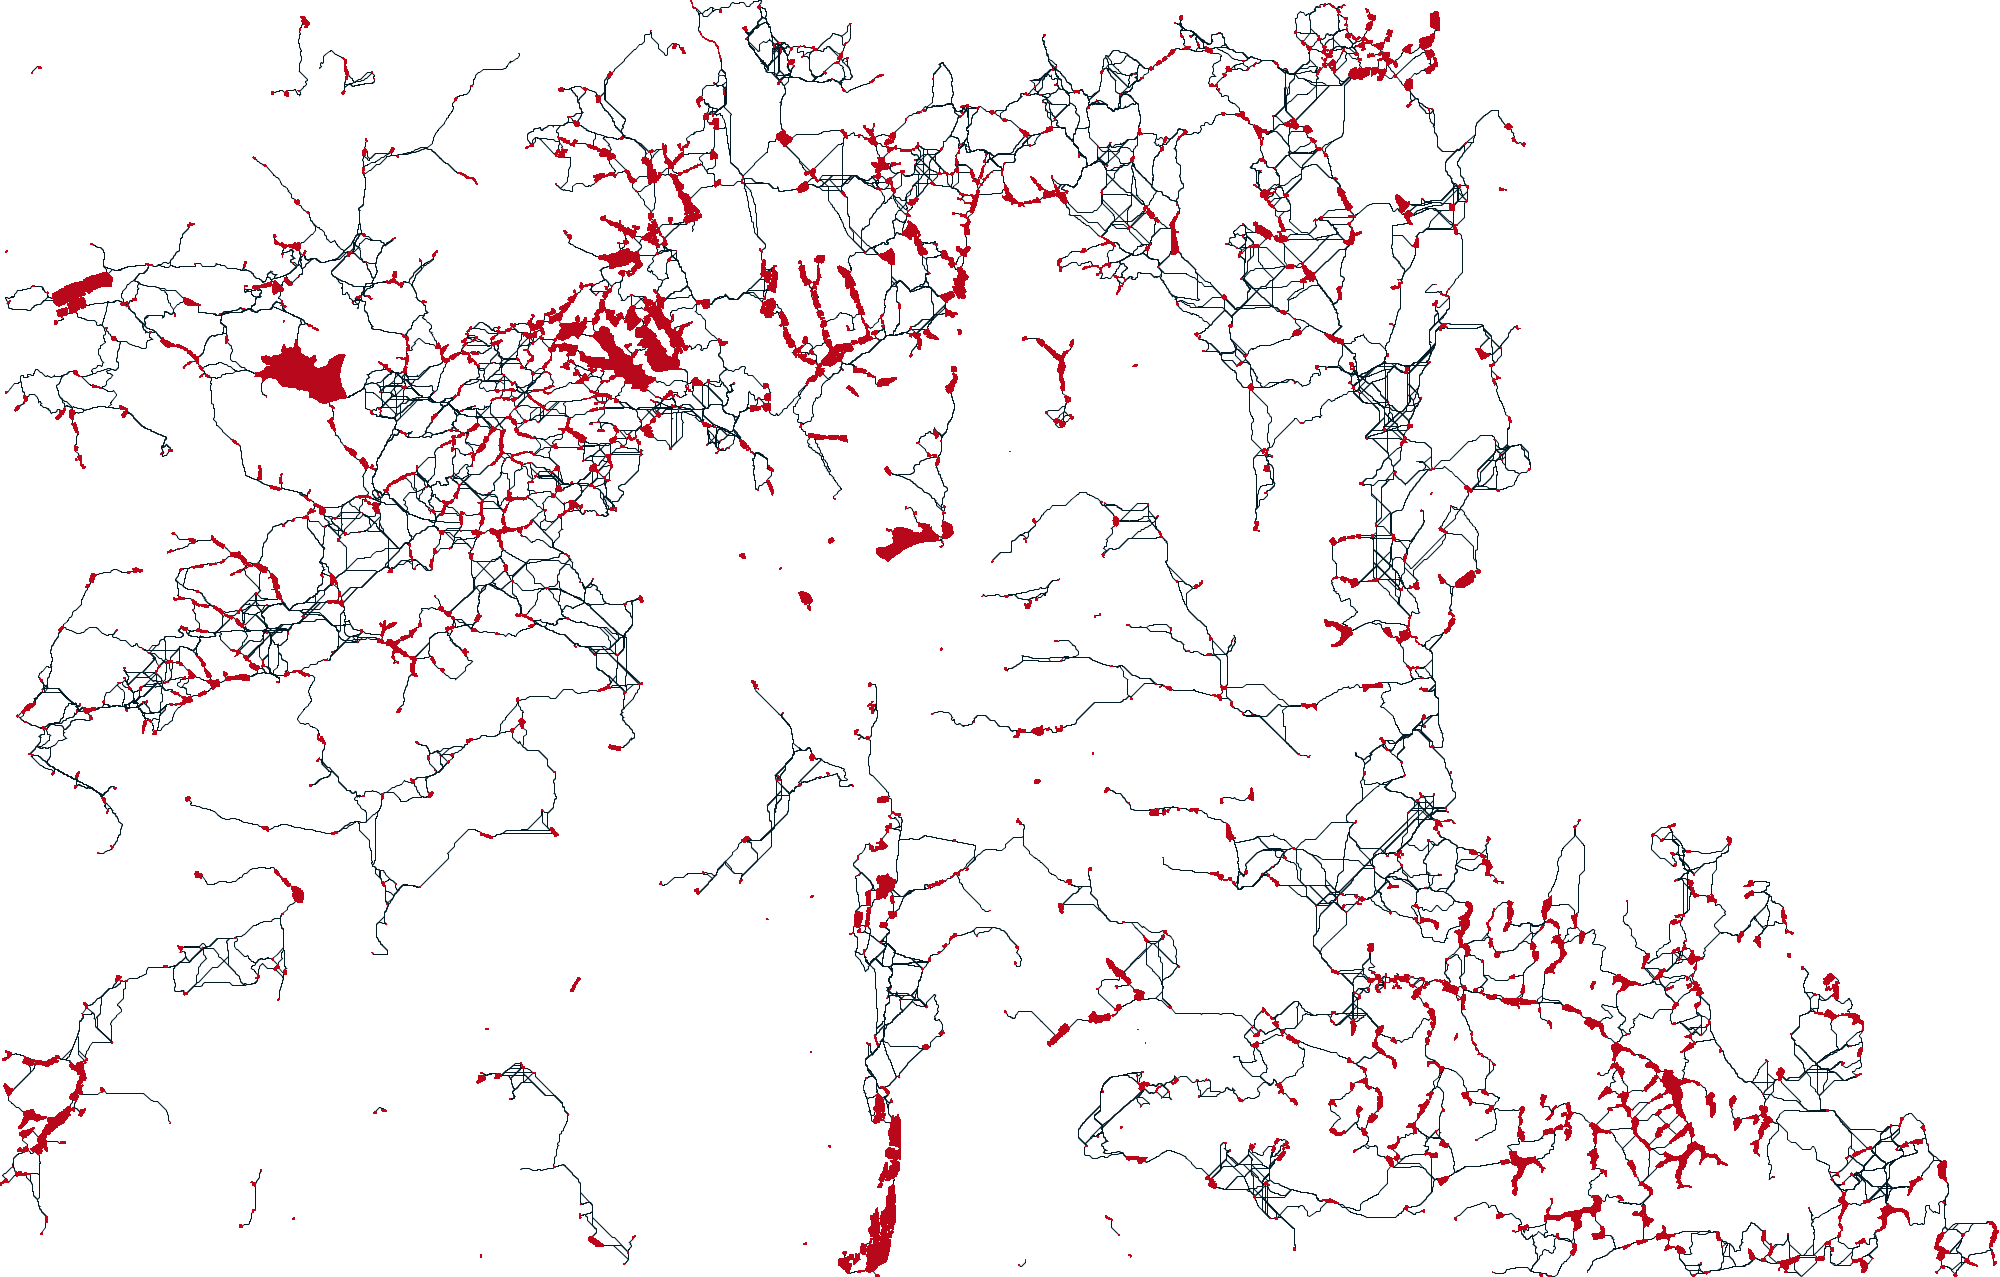
\includegraphics[scale=0.1]{img/manual-en_img17.png}
	\caption*{Left: Topologic view - Right: Realistic view}
\end{figure}


The Remove entry can be used to remove the selected graph. The project is saved automatically.

Properties displays the parameters used in constructing the graph: graph name, graph type with the possible maximum distance used, and the number of links.

The OD Matrix (Origin–Destination Matrix) entry creates a table with the distance between each pair of nodes for the given graph. The unit of distance depends on the type of distance used in the graph. The absence of any connection between two nodes is noted NaN (Not a Number). This matrix is saved in the project file in text format named: “graph name-
odmatrix.txt~”.

\subsection{Object properties}
\label{properties}
The properties of link sets, graph elements (nodes, links, and components), and point data are available by right-clicking on each of them.

The Style menu includes the display parameters for objects: color, line width, label, symbol size (for nodes only). Objects can be represented in the same way (single symbol) or according to some attribute. A discretization method can be applied to classify objects according to the values of the selected attribute. By default, the legend of objects is displayed in the table of contents. It can be masked by unchecking
the Legend button.

The Export~menu can be used to export objects to a shapefile (*.shp), a geopackage (.gpkg) or a text file (*.txt).

The Statistic menu displays the distribution of the values of one or more attributes:
\begin{itemize}
	\item scatter plot: values of two attributes are plotted on a two-dimensional graph,
	\item histogram: the bar chart of the values of an attribute is generated.
\end{itemize}

It is also possible to display the values of a given object by selecting it with the white arrow. After selection, the values of attributes are displayed in a new right-hand column named “feature properties”. This column can be closed by clicking on the Properties menu in the top bar.

\begin{figure}[H]
	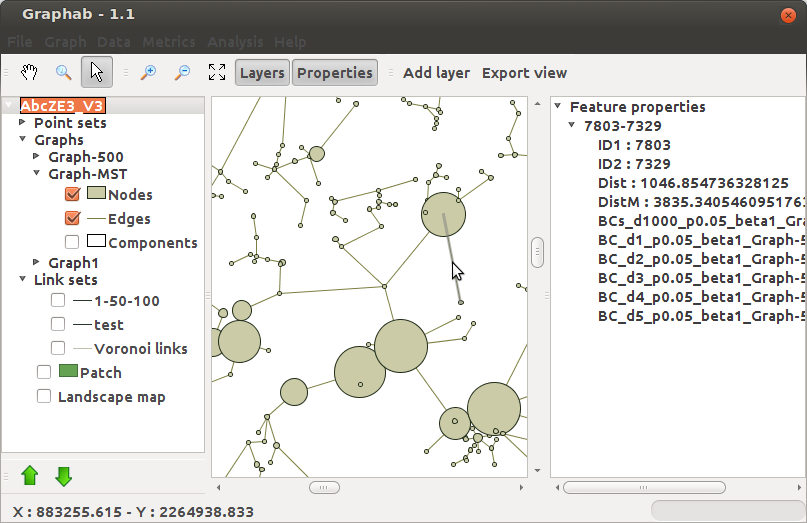
\includegraphics[scale=0.5]{img/manual-en_img18.png}
\end{figure}


\section{Processing capabilities and limitations}
\label{limit}
Graph-based methods provide an efficient modeling framework, but they can raise a question of computing capacity. Two specific points have received particular attention in Graphab: (1) calculation of link sets, (2) calculation of connectivity metrics. All these computations have been optimized by parallelization. This development mode improves computational efficiency by using a multi-processor architecture, a
quad-core processor being theoretically four times faster than a single-core processor.

In \cite{2012_graphab_EMS}, several tests were conducted to measure the computational capacity of Graphab in different configurations. Three configurations were compared for these
tests: (1) one core (3 Go RAM) corresponding to a current desktop computer, (2) four cores (6 Go RAM) corresponding to a workstation, and (3) 20 cores (15 Go RAM) corresponding to a server. The landscape map used was a grid of 14000*18000 pixels (252 millions of pixels) representing the landscape elements of the region of Franche-Comté (France) at a spatial resolution of 10 m. The landscape map contained 22,634 habitat patches. 

\begin{table}[H]
\begin{tabular}{|l|l|l|l|l|}
\hline
Topology & Distance & Current desktop & Workstation  & Server\\
\hline
Complete
 & Euclidean & 1927s (32 min) & 516s (8 min) & 133s (2 min)\\
\hhline{~----}
 & Least-cost & 19252s (5h 21 min) & 4301s (1h 11 min) & 1037s (17 min)\\
\hline
Planar
 & Euclidean & 43s & 12s & 2.6s\\
\hhline{~----}
 & Least-cost & 1080s (18 min) & 295s (5 min) & 82s (1 min)\\
\hline
\end{tabular}
\caption{Computation times (seconds) required for calculating several link sets}
\label{perf}
\end{table}

The memory used by the software plays an important role. If there is not enough RAM, computation will be slower or may fail (OutOfMemoryError or GC Overhead message). The File/ Preferences / Memory menu can be used to adjust the memory allocated to Graphab. If you have a 32-bit version of Java, Graphab will be limited to about 2 Go (2000 Mo) of memory. If your computer has more than 2 Go of RAM memory, it is highly
recommended you install the 64-bit version of Java to use the available memory beyond 2 Go.


\section{Metrics}


\begin{table}[H]
\begin{tabular}{|c|l|l|c|c|c|c|}
	\hline
	Family & Connectivity metrics & Code & \multicolumn{3}{m{3.6cm}|}{\centering Computing level} & Delta metrics\\
	\hhline{~~~---~}
	& & & Global & Comp. & Local &\\
	\hline
	Weighted
	& \nameref{metric_F} & F & × & × & × &\\
	\hhline{~------}
	& \nameref{metric_EC} & EC & × & × &  & ×\\
	\hhline{~------}
	& \nameref{metric_PC} & PC & × & × &  & ×\\
	\hhline{~------}
	& \nameref{metric_IF}  & IF &  &  & × &\\
	\hhline{~------}
	& \nameref{metric_dPC} & dPC &  &  &  & ×\\
	\hhline{~------} 
	& \nameref{metric_BC} & BC &  &  & × & \\
	\hhline{~------}
	& \nameref{metric_IIC} & IIC & × & × &  & × \\
	\hhline{~------}	
	& \nameref{metric_CF} & CF &  &  & × & \\
	\hline
	Area
	& \nameref{metric_MSC} & MSC & × &  &  & \\
	\hhline{~------}
	& \nameref{metric_SLC} & SLC & × &  &  & \\
	\hhline{~------}
	& \nameref{metric_CCP} & CCP & × &  &  & \\
	\hhline{~------}
	& \nameref{metric_ECS} & ECS & × &  &  & \\
	\hline
	Topological
	& \nameref{metric_Dg} & Dg &  &  & × & \\
	\hhline{~------}
	& \nameref{metric_CC}  & CC &  &  & × & \\
	\hhline{~------}
	& \nameref{metric_CCe} & CCe &  &  & × & \\
	\hhline{~------}
	& \nameref{metric_Ec} & Ec &  &  & × & \\
	\hhline{~------}
	& \nameref{metric_CCor} & CCor &  &  & × & \\
	\hhline{~------}
	& \nameref{metric_NC} & NC & × &  &  & \\
	\hhline{~------}
	& \nameref{metric_GD} & GD & × & × &  & ×\\
	\hhline{~------}
	& \nameref{metric_H} & H & × & × &  & ×\\
	\hhline{~------}
	& \nameref{metric_W} & W & × &  &  & \\
	\hline
\end{tabular}
\caption{Summary table of metrics in Graphab}
\end{table}

\bigskip

\begin{table}[H]
	\begin{tabular}{|m{2cm}|m{13cm}|}
		\hline
		Terms & Meaning\\\hline
		$n$	& Number of patches\\\hline
		$nc$ & Number of components\\\hline
		${n}_{k}$ &	Number of patches in the component k\\\hline
		${N}_{i}$ &	All patches close to the patch i\\\hline
		${a}_{i}$ &	Capacity of the patch i (generally the surface area)\\\hline
		${ac}_{k}$ & Capacity of the component k (sum of the capacity of the patches composing k)\\\hline
		$A$	& Area of the study zone \\\hline
		${d}_{ij}$ & Distance between the patches i and j (generally the least-cost distance between them) \\\hline
		${e}^{-\alpha {d}_{ij}}$ & Probability of movement between the patches i and j\\\hline
		$\alpha$ & Brake on movement distance  \\\hline
		$\beta$	& Exponent to weight more or less capacity\\\hline
	\end{tabular}
	\caption{Mathematical terms used}
\end{table}


\subsection{Weighted metrics}
\label{weight_metric}
\subsubsection{Flux}
\label{metric_F}
\begin{table}[H]
\begin{tabular}{|m{3.24cm}|m{4.4810004cm}m{7.924cm}|}
\hline 
Flux ($F$) &  \multicolumn{1}{m{4.4810004cm}|}{Formula} &
Meaning\\\hline
Global level &
\multicolumn{1}{m{4.4810004cm}|}{\begin{equation*}
S\#F=\sum _{i=1}^{n}{\sum
_{\begin{matrix}j=1\\j{\neq}i\end{matrix}}^{n}{{a}_{j}^{\beta
}}}{e}^{-\alpha {d}_{\mathit{ij}}}
\end{equation*}
} &
For the entire graph: sum of potential dispersions from all
patches.\\\hline
Local level &
\multicolumn{1}{m{4.4810004cm}|}{\begin{equation*}
{F}_{i}=\sum
_{\begin{matrix}j=1\\j{\neq}i\end{matrix}}^{n}{{a}_{j}^{\beta
}}{e}^{-\alpha {d}_{\mathit{ij}}}
\end{equation*}
} &
For the focal patch $i$ : sum of capacity of patches other than i and
weighted according to their minimum distance to the focal patch through
the graph. This sum is an indicator of the potential dispersion from
the patch $i$ or, conversely to the patch $i$.\\\hline
Values &
\multicolumn{2}{m{12.6050005cm}|}{
Values depend on the definition of $a$.
If $a$ represents an area, F expresses an area.

Minimum value: 0

Maximum value: Total area of habitat 
}\\\hline
Comment &
\multicolumn{2}{m{12.6050005cm}|}{The path used in the graph is the one
that maximizes  ${e}^{-\mathit{\alpha d}}$, i.e. the one that minimizes
the distance d (or the cost) between the patches i and j. 

This metric is called Area Weighted Flux (AWF) in some publications.
However in Graphab, a is more general because it represents patch
capacity, which may be their area or some other criterion chosen by the
user. Similarly, the weighting is variable depending on the $\beta $
parameter. In CS22, AWF is calculated only from patches directly
connected to the focal patch, while Graphab takes into account
indirectly connected patches.

}\\\hline
References &
\multicolumn{2}{m{12.6050005cm}|}{
\cite{Urban2001} \cite{Saura2009} \cite{2012_SDM}
}\\\hline
\end{tabular}
\end{table}

\subsubsection{Equivalent Connectivity}
\label{metric_EC}
\begin{table}[H]
\begin{tabular}{|m{3.24cm}|m{4.4810004cm}m{7.924cm}|}
\hline
Equivalent Connectivity ($EC$) &
\multicolumn{1}{m{4.4810004cm}|}{Formula} &
Meaning\\\hline
Global level 

Component level

Delta &
\multicolumn{1}{m{4.4810004cm}|}{\begin{equation*}
\mathit{EC}=\sqrt{\sum _{i=1}^{n}{\sum _{j=1}^{n}{{a}_{i}}}{{a}_{j}e}^{-\alpha {d}_{\mathit{ij}}}}
\end{equation*}
} &
Square root of the sum of products of capacity of all pairs of patches weighted by their interaction probability. \\\hline
Values &
\multicolumn{2}{m{12.6050005cm}|}{Unit corresponds to the capacity unit of the patches.
	
Minimum value: 0

Maximum value: sum of capacities
}\\\hline
Comment &
\multicolumn{2}{m{12.6050005cm}|}{For each pair of patches, the path of
the graph used is the one that maximizes ${e}^{-\mathit{\alpha d}}$,
i.e. the one that minimizes the distance $d$ (or the cost) between the
patches $i$ and $j$.

}\\\hline
Reference &
\multicolumn{2}{m{12.6050005cm}|}{
\cite{Saura2011}
}\\\hline
\end{tabular}
\end{table}

\subsubsection{Probability of Connectivity}
\label{metric_PC}
\begin{table}[H]
	\begin{tabular}{|m{3.24cm}|m{4.4810004cm}m{7.924cm}|}
		\hline
		Probability of Connectivity ($PC$) &
		\multicolumn{1}{m{4.4810004cm}|}{Formula} &
		Meaning\\\hline
		Global level 
		
		Component level
		
		Delta &
		\multicolumn{1}{m{4.4810004cm}|}{\begin{equation*}
			\mathit{PC}=\frac{1}{{A}^{2}}\sum _{i=1}^{n}{\sum
				_{j=1}^{n}{{a}_{i}}}{{a}_{j} e}^{-\alpha
				{d}_{\mathit{ij}}}
			\end{equation*}
		} &
		Sum of products of capacity of all pairs of patches weighted by their interaction probability, divided by the square of the area of the study zone. This ratio is the equivalent to the probability that two points randomly placed in the study area are connected.\\\hline
		Values &
		\multicolumn{2}{m{12.6050005cm}|}{Values correspond to a probability.
			
			Minimum value: 0
			
			Maximum value: 1
		}\\\hline
		Comment &
		\multicolumn{2}{m{12.6050005cm}|}{For each pair of patches, the path of
			the graph used is the one that maximizes ${e}^{-\mathit{\alpha d}}$,
			i.e. the one that minimizes the distance $d$ (or the cost) between the
			patches $i$ and $j$.
			
			This metric is not available when $a_i$ does not represent patch area.
		}\\\hline
		Reference &
		\multicolumn{2}{m{12.6050005cm}|}{
			\cite{Saura2007}
		}\\\hline
	\end{tabular}
\end{table}

\subsubsection{Interaction Flux (replace FPC)}
\label{metric_IF}
\begin{table}[H]
\begin{tabular}{|m{3.24cm}|m{4.4810004cm}m{7.924cm}|}
\hline
Interaction Flux
($IF$) &
\multicolumn{1}{m{4.4810004cm}|}{Formula} &
Meaning\\\hline
Local level &
\multicolumn{1}{m{4.4810004cm}|}{\begin{equation*}
{\mathit{IF}}_{i}=\sum _{j=1}^{n}{{{a}_{i}^{\beta }{a}_{j}^{\beta }e}^{-\alpha {d}_{\mathit{ij}}}}
\end{equation*}
} &
Sum of products of the focal patch capacity with all the other patches,
weighted by their interaction probability.\\\hline
Values &
\multicolumn{2}{m{12.6050005cm}|}{
Minimum value: 0

Maximum value: sum of capacities
}\\\hline
Comment &
\multicolumn{2}{m{12.6050005cm}|}{For each pair of patches, the path of
the graph used is one that maximizes ${e}^{-\mathit{\alpha d}}$, i.e.
one that minimizes the distance $d$ (or the cost) between the patches $i$
and $j$.

This metric corresponds to the local contribution of a patch in the $PC$ index, since  $\mathit{PC}=\frac{1}{A^2}\sum _{i}{{\mathit{IF}}_{i}}$, with $\beta = 1$. 

It is the equivalent of ${dPC}_{flux}+{dPC}_{area}$ not divided
by the global value of $PC$. However, the $IF$ metric is obtained faster because it is not calculated on the basis of patch removal (delta mode).
}\\\hline
References &
\multicolumn{2}{m{12.6050005cm}|}{\cite{2014_LUP},\cite{2017_landmod}}\\\hline
\end{tabular}
\end{table}

\subsubsection{Fractions of delta Probability of Connectivity}
\label{metric_dPC}
\begin{table}[H]
\begin{tabular}{|m{2.4919999cm}|m{5.229cm}m{7.924cm}|}
\hline
\multicolumn{3}{|m{16.044998cm}|}{Fractions of delta Probability of
Connectivity ($dPC$, $dPC_{area}$, $dPC_{flux}$, $dPC_{connector}$)}\\\hline
 &
\multicolumn{1}{m{5.229cm}|}{Formula} &
Meaning\\\hline
Delta &
\multicolumn{1}{m{5.229cm}|}{\begin{equation*}
{\mathit{dPC}}_{i}=\frac{(\mathit{PC}-{\mathit{PC}}_{i}^{'})}{\mathit{PC}}
\end{equation*}
\begin{equation*}
{{\mathit{dPC}}_{i}=\mathit{dPC}}_{\mathit{area}}+{\mathit{dPC}}_{\mathit{flux}}{+\mathit{dPC}}_{\mathit{connector}}
\end{equation*}
\begin{equation*}
{\mathit{dPC}}_{\mathit{area}}=\frac{{a}_{i}^{2}}{{A}^{2}\mathit{PC}}
\end{equation*}
\begin{equation*}
{dPC}_{flux}=\frac{{IF}_{i}}{PC}-{dPC}_{area}
\end{equation*}
} &
Rate of variation between the value of PC index and the value of PC’
corresponding to the removal of the patch i.

The value of $dPC$ is decomposed into three parts:

{}- $dPC_{area}$ is the variation induced by the area lost after removal;

{}- $dPC_{flux}$ is the variation induced by the loss of interaction between
the patch i and other patches;

{}- $dPC_{connector}$ is the variation induced by the modification of paths
connecting other patches and initially routed through i.~\\\hline
Values &
\multicolumn{2}{m{13.353cm}|}{
Minimum value: 0

Maximum value: 1
}\\\hline
Comment &
\multicolumn{2}{m{13.353cm}|}{

If $a$ does not represent patch area, $dPC_{area}$ does not express a loss of area but a loss of capacity.

}\\\hline
Reference &
\multicolumn{2}{m{13.353cm}|}{\cite{Saura2010}}\\\hline
\end{tabular}
\end{table}


\subsubsection{Betweenness Centrality index}
\label{metric_BC}
\begin{table}[H]
\begin{tabular}{|m{3.24cm}|m{4.4810004cm}m{7.924cm}|}
\hline
Betweenness Centrality index
($BC$) &
\multicolumn{1}{m{4.4810004cm}|}{Formula} &
Meaning\\\hline
Local level &
\multicolumn{1}{m{4.4810004cm}|}{\begin{equation*}
{\mathit{BC}}_{i}=\sum _{j}{\sum _{k}{{a}_{j}^{\beta }}}{a}_{k}^{\beta
}{e}^{-\alpha {d}_{\mathit{jk}}}
\end{equation*}
\begin{equation*}
j,k{\in}\left\{1..n\right\},k<j,i{\in}{P}_{\mathit{jk}}
\end{equation*}
} &
Sum of the shortest paths through the focal patch i, each path is
weighted by the product of the capacities of the patches connected and
of their interaction probability.

Pjk represents all the patches crossed by the shortest path between the
patches j and k.

\\\hline
Values &
\multicolumn{2}{m{12.6050005cm}|}{Values depend on the configuration.
They correspond to a weight of potential transit.

Minimum value: 0

Maximum value: square of the total area of habitat.
}\\\hline
Comment &
\multicolumn{2}{m{12.6050005cm}|}{With an adjustment of $\alpha = 0$
and $\beta = 0$ (uniform weighting of paths), the $BC$ index is the same
as that used in other types of graphs. 

An adjustment of $\alpha = 0$ and $\beta = 1$ gives paths a weight
proportional to the product of the capacities of the patches that they
connect, whatever their distance. 

In \cite{2012_graphab_EMS, 2012_SDM}, the $BC_l$ index was proposed so as to
give greater weight to paths exceeding a given criterion (e.g.
dispersal distance). But tests showed that this index was strongly
correlated with the weighted $BC$ adjusted with $\alpha=0$. 

In \cite{Bodin2010}, the  ${\mathit{BC}}_{\mathit{pc}}$ is the
weighted BC with d equal to the dispersal distance,  $\alpha $ as 
${e}^{-\mathit{\alpha d}}=0.05$ and  $\beta =1$.

}\\\hline
Reference &
\multicolumn{2}{m{12.6050005cm}|}{
\cite{Bodin2010}
\cite{2012_graphab_EMS}	
}\\\hline
\end{tabular}
\end{table}


\subsubsection{Integral Index of Connectivity}
\label{metric_IIC}
\begin{table}[H]
\begin{tabular}{|m{3.24cm}|m{4.4810004cm}m{7.924cm}|}
\hline
Integral Index of Connectivity
($IIC$) &
\multicolumn{1}{m{4.4810004cm}|}{Formula} &
Meaning\\\hline
Global level

Component level

Delta &
\multicolumn{1}{m{4.4810004cm}|}{\begin{equation*}
\mathit{IIC}=\frac{1}{{A}^{2}}\sum _{i=1}^{n}{\sum
_{j=1}^{n}{{\frac{{a}_{i}{a}_{j}}{{1+\mathit{nl}}_{\mathit{ij}}}}}}
\end{equation*}
} &
For the entire graph: product of patch capacities divided by the number
of links between them, the sum is divided by the square of the area of
the study zone.

IIC is built like the PC index but using the inverse of a topological
distance rather than a negative exponential function of the distance
based on the link impedance.

\\\hline
Values &
\multicolumn{2}{m{12.6050005cm}|}{Minimum value: 0

Maximum value: 1
}\\\hline
Reference &
\multicolumn{2}{m{12.6050005cm}|}{\cite{Pascual2006}}\\\hline
\end{tabular}
\end{table}

\subsubsection{Current Flow}
\label{metric_CF}
\begin{table}[H]
	\begin{tabular}{|m{3.24cm}|m{4.4810004cm}m{7.924cm}|}
		\hline
		Current Flow ($CF$) &
		\multicolumn{1}{m{4.4810004cm}|}{Formula} &
		Meaning\\\hline
		Local level &
		\multicolumn{1}{m{4.4810004cm}|}{
			\begin{equation*}
			CF_{i}=\sum_{j}^n{c_i^j}
			\end{equation*}
		} &
		Sum of currents passing through the patch $i$.
		
		$c_i^j$ represents the current through the patch $i$ when currents are sent from all patches (except $j$) to the patch $j$. The patch $j$ is connected to the ground.
		
		\\\hline
		Values &
		\multicolumn{2}{m{12.6050005cm}|}{			
			Minimum value : 0
			
			Maximum value : $(n-1)(n-2)$ if $\beta=0$
			
			$(n-2)\sum_i^{n-1} a_i$ if $\beta=1$
			
		}\\\hline
		Comment &
		\multicolumn{2}{m{12.6050005cm}|}{
			The $CF$ metric uses the electrical circuit theory. Each link of the graph corresponds to a resistor, the current sources and the ground are attached to the patches.
			
			If $\beta=0$, each patch emits a current of 1, if $\beta=1$, each patch emits a current equals to its capacity.
			
			This metric can be seen as an equivalent of $BC$ metric (with $\alpha=0$ and $\beta=0$) that considers all possible paths, not just the shortest one.
			
		}\\\hline
		Reference &
		\multicolumn{2}{m{12.6050005cm}|}{		
			\cite{2015_collisions}
		}\\\hline
	\end{tabular}
\end{table}

\subsection{Area metrics}

\subsubsection{Mean Size of the Components}
\label{metric_MSC}
\begin{table}[H]
\begin{tabular}{|m{3.24cm}|m{4.4810004cm}m{7.924cm}|}
\hline
Mean Size of the Components ($MSC$) &
\multicolumn{1}{m{4.4810004cm}|}{Formula} &
Meaning\\\hline
Global level &
\multicolumn{1}{m{4.4810004cm}|}{\begin{equation*}
\mathit{MSC}=\frac{1}{\mathit{nc}}\sum
_{k=1}^{\mathit{nc}}{{\mathit{ac}}_{k}}
\end{equation*}
} &
Mean of the component capacities.

\\\hline
Values &
\multicolumn{2}{m{12.6050005cm}|}{Minimum value: minimum capacity

Maximum value:  $\mathit{SLC}$
}\\\hline
\end{tabular}
\end{table}


\subsubsection{Size of the Largest Component}
\label{metric_SLC}
\begin{table}[H]
\begin{tabular}{|m{3.24cm}|m{4.4810004cm}m{7.924cm}|}
\hline
Size of the Largest Component
($SLC$) &
\multicolumn{1}{m{4.4810004cm}|}{Formula} &
Meaning\\\hline
Global level &
\multicolumn{1}{m{4.4810004cm}|}{\begin{equation*}
\mathit{SLC}=\mathit{max}\{{\mathit{ac}}_{k}\}
\end{equation*}
} &
Largest capacity of components.

\\\hline
Values &
\multicolumn{2}{m{12.6050005cm}|}{Minimum value: minimum capacity

Maximum value: maximum capacity
}\\\hline
\end{tabular}
\end{table}


\subsubsection{Class Coincidence Probability}
\label{metric_CCP}
\begin{table}[H]
\begin{tabular}{|m{3.24cm}|m{4.4810004cm}m{7.924cm}|}
\hline
Class Coincidence Probability
($CCP$) &
\multicolumn{1}{m{4.4810004cm}|}{Formula} &
Meaning\\\hline
Global level &
\multicolumn{1}{m{4.4810004cm}|}{\begin{equation*}
\mathit{CCP}=\sum
_{k=1}^{\mathit{nc}}{{\left(\frac{{\mathit{ac}}_{k}}{\sum
_{l}{{\mathit{ac}}_{l}}}\right)}^{2}}
\end{equation*}
} &
Probability that two points randomly placed on the
graph belong to the same component.\\\hline
Values &
\multicolumn{2}{m{12.6050005cm}|}{Minimum value: $\rightarrow 0$ (as many components as patches and regular capacities)

Maximum value: 1 (only one component)

}\\\hline
Reference &
\multicolumn{2}{m{12.6050005cm}|}{\cite{Pascual2006}}\\\hline
\end{tabular}
\end{table}


\subsubsection{Expected Cluster Size}
\label{metric_ECS}
\begin{table}[H]
\begin{tabular}{|m{3.24cm}|m{4.4810004cm}m{7.924cm}|}
\hline
Expected Cluster Size ($ECS$) &
\multicolumn{1}{m{4.4810004cm}|}{Formula} &
Meaning\\\hline
Global level &
\multicolumn{1}{m{4.4810004cm}|}{\begin{equation*}
\mathit{ECS}=\frac{1}{\sum _{k}{{\mathit{ac}}_{k}}}\sum
_{k=1}^{\mathit{nc}}{{{\mathit{ac}}_{k}^{2}}}
\end{equation*}
} &
Expected size of a component 

\\\hline
Values &
\multicolumn{2}{m{12.6050005cm}|}{Minimum value: minimum capacity (as many components as patches and regular capacities)

Maximum value: sum of capacities (only one component)

}\\\hline
Reference &
\multicolumn{2}{m{12.6050005cm}|}{\cite{OBrien2006}}\\\hline
\end{tabular}
\end{table}


\subsection{Topological metrics}

\subsubsection{Wilks' Lambda}
\label{metric_W}
\begin{table}[H]
	\begin{tabular}{|m{3.24cm}|m{4.4810004cm}m{7.924cm}|}
		\hline
		Wilks' Lambda ($W$) &
		\multicolumn{1}{m{4.4810004cm}|}{Formula} &
		Meaning\\\hline
		Global level &
		\multicolumn{1}{m{4.4810004cm}|}{\begin{equation*}
				W_{Lambda}=\frac{|W|}{|T|}
			\end{equation*}
		} &
		Ratio between within-classes (within-components) (co)variance $|W|$ and total (co)variance $|T|$
		
		\\\hline
		Values &
		\multicolumn{2}{m{12.6050005cm}|}{Minimum value: 0 the patches belonging to the same component are identical for all the variables (\textit{i.e.} perfect partition)
			
			Maximum value: 1 patches belonging to the same component differ as much as with the other patches (\textit{i.e.} meaning an irrelevant partition)
			
		}\\\hline
		Reference &
		\multicolumn{2}{m{12.6050005cm}|}{\cite{Everitt2001}, \cite{2017_clustering}}\\\hline
	\end{tabular}
\end{table}


\subsubsection{Harary Index}
\label{metric_H}
\begin{table}[H]
\begin{tabular}{|m{3.24cm}|m{4.4810004cm}m{7.924cm}|}
\hline
Harary Index ($H$) &
\multicolumn{1}{m{4.4810004cm}|}{Formula} &
Meaning\\\hline
Global level

Component level

Delta  &
\multicolumn{1}{m{4.4810004cm}|}{\begin{equation*}
H=\frac{1}{2}\sum _{i=1}^{n}{\sum
_{\begin{matrix}j=1\\j{\neq}i\end{matrix}}^{n}{\frac{1}{{\mathit{nl}}_{\mathit{ij}}}}}
\end{equation*}
} &
Sum of the inverse of the number of links between all pairs of patches.

\\\hline
Values &
\multicolumn{2}{m{12.6050005cm}|}{Minimum value: 0 for a graph with no edges

Maximum value: $\frac{n(n-1)}{2}$ for a complete graph

}\\\hline
Comment &
\multicolumn{2}{m{12.6050005cm}|}{For pairs of patches not connected by
a path, we have :   ${\mathit{nl}}_{\mathit{ij}}=+{\infty}$}\\\hline
Reference &
\multicolumn{2}{m{12.6050005cm}|}{\cite{Ricotta2000}}\\\hline
\end{tabular}
\end{table}


\subsubsection{Graph Diameter}
\label{metric_GD}
\begin{table}[H]
\begin{tabular}{|m{3.24cm}|m{4.4810004cm}m{7.924cm}|}
\hline
Graph Diameter ($GD$) &
\multicolumn{1}{m{4.4810004cm}|}{Formula} &
Meaning\\\hline
Global level

Component level 

Delta &
\multicolumn{1}{m{4.4810004cm}|}{\begin{equation*}
\mathit{GD}=\underset{\mathit{ij}}{\mathit{max}}{d}_{\mathit{ij}}
\end{equation*}
\begin{equation*}
\mathit{GD}=\underset{i}{\mathit{max}}{\mathit{Ec}}_{i}
\end{equation*}
} &
Greatest distance between two patches of the graph. \\\hline
Values &
\multicolumn{2}{m{12.6050005cm}|}{Minimum value: 0

Maximum value:  $+{\infty}$

}\\\hline
Comment &
\multicolumn{2}{m{12.6050005cm}|}{When the nodes i and j are not related
 ${d}_{\mathit{ij}}=0$

This metric is the global version of the metric  ${\mathit{Ec}}_{i}$

}\\\hline
Reference &
\multicolumn{2}{m{12.6050005cm}|}{\cite{Urban2001}
}\\\hline
\end{tabular}
\end{table}


\subsubsection{Number of Components}
\label{metric_NC}
\begin{table}[H]
\begin{tabular}{|m{3.24cm}|m{4.4810004cm}m{7.924cm}|}
\hline
Number of Components ($NC$) &
\multicolumn{1}{m{4.4810004cm}|}{Formula} &
Meaning\\\hline
Global  level

 &
\multicolumn{1}{m{4.4810004cm}|}{\begin{equation*}
\mathit{NC}=\mathit{nc}
\end{equation*}
} &
Number of components of the graph.\\\hline
Values &
\multicolumn{2}{m{12.6050005cm}|}{Minimum value: 1

Maximum value :  $n$

}\\\hline
Reference &
\multicolumn{2}{m{12.6050005cm}|}{\cite{Urban2001}
}\\\hline
\end{tabular}
\end{table}


\subsubsection{Node Degree}
\label{metric_Dg}
\begin{table}[H]
\begin{tabular}{|m{3.24cm}|m{4.4810004cm}m{7.924cm}|}
\hline
Node Degree ($Dg$) &
\multicolumn{1}{m{4.4810004cm}|}{Formula} &
Meaning\\\hline
Local level

 &
\multicolumn{1}{m{4.4810004cm}|}{\begin{equation*}
{\mathit{Dg}}_{i}=\left|{N}_{i}\right|
\end{equation*}
} &
Number of edges connected to the node $i$ \textit{ie.}
number of patches connected directly to the patch $i$\\\hline
Values &
\multicolumn{2}{m{12.6050005cm}|}{Minimum value: 0

Maximum value:  $n$

}\\\hline
Comment &
\multicolumn{2}{m{12.6050005cm}|}{There is an equivalence between the
node degree and the number of nearest patches because graphs are not
oriented and do not contain any loops.

}\\\hline
Reference &
\multicolumn{2}{m{12.6050005cm}|}{Freeman, 1979}\\\hline
\end{tabular}
\end{table}


\subsubsection{Clustering Coefficient}
\label{metric_CC}
\begin{table}[H]
\begin{tabular}{|m{3.24cm}|m{5.303cm}m{7.103cm}|}
\hline
Clustering Coefficient ($CC$) &
\multicolumn{1}{m{5.303cm}|}{Formula} &
Meaning\\\hline
Local level

 &
\multicolumn{1}{m{5.303cm}|}{\begin{equation*}
{\mathit{CC}}_{i}=\frac{1}{\left|{N}_{i}\right|\left(\left|{N}_{i}\right|-1\right)}\sum
_{j{\in}{N}_{i}}{\left|{N}_{i}{\cap}{N}_{j}\right|}
\end{equation*}
} &
Ratio of the number of nodes close to i which are neighbors to each
other over the possible total. \\\hline
Values &
\multicolumn{2}{m{12.606cm}|}{Minimum value: 0

Maximum value: 1

}\\\hline
Comment &
\multicolumn{2}{m{12.606cm}|}{Si 
$\left|{N}_{i}\right|{\leq}1\rightarrow {\mathit{CC}}_{i}=0$ }\\\hline
Reference &
\multicolumn{2}{m{12.606cm}|}{\cite{Ricotta2000}}\\\hline
\end{tabular}
\end{table}


\subsubsection{Closeness Centrality}
\label{metric_CCe}
\begin{table}[H]
\begin{tabular}{|m{3.24cm}|m{4.4810004cm}m{7.924cm}|}
\hline
Closeness Centrality ($CCe$) &
\multicolumn{1}{m{4.4810004cm}|}{Formula} &
Meaning\\\hline
Local level

 &
\multicolumn{1}{m{4.4810004cm}|}{\begin{equation*}
{\mathit{CCe}}_{i}=\frac{1}{{n}_{k}-1}\sum
_{\begin{matrix}j=1\\j{\neq}i\end{matrix}}^{{n}_{k}}{{d}_{\mathit{ij}}}
\end{equation*}
} &
Mean distance from the patch i to all other patches of its component k.
\\\hline
Values &
\multicolumn{2}{m{12.6050005cm}|}{Minimum value: 0

Maximum value:  $+{\infty}$

}\\\hline
Comment &
\multicolumn{2}{m{12.6050005cm}|}{Si  ${n}_{k}=1\rightarrow
{\mathit{CCe}}_{i}=0$ }\\\hline
Reference &
\multicolumn{2}{m{12.6050005cm}|}{Freeman, 1979}\\\hline
\end{tabular}
\end{table}


\subsubsection{Eccentricity}
\label{metric_Ec}
\begin{table}[H]
\begin{tabular}{|m{3.24cm}|m{4.4810004cm}m{7.924cm}|}
\hline
Eccentricity ($Ec$) &
\multicolumn{1}{m{4.4810004cm}|}{Formula} &
Meaning\\\hline
Local level

 &
\multicolumn{1}{m{4.4810004cm}|}{\begin{equation*}
{\mathit{Ec}}_{i}=\underset{j}{\mathit{max}}{d}_{\mathit{ij}}
\end{equation*}
} &
Maximum distance from the patch i to another patch of its component k.
\\\hline
Values &
\multicolumn{2}{m{12.6050005cm}|}{Minimum value: 0

Maximum value:  $+{\infty}$

}\\\hline
Reference &
\multicolumn{2}{m{12.6050005cm}|}{\cite{Urban2001}
}\\\hline
\end{tabular}
\end{table}


\subsubsection{Connectivity Correlation}
\label{metric_CCor}
\begin{table}[H]
\begin{tabular}{|m{3.24cm}|m{4.4810004cm}m{7.924cm}|}
\hline
Connectivity correlation ($CCor$) &
\multicolumn{1}{m{4.4810004cm}|}{Formula} &
Meaning\\\hline
Local level

 &
\multicolumn{1}{m{4.4810004cm}|}{\begin{equation*}
{\mathit{CCor}}_{i}=\frac{{\left|{N}_{i}\right|}^{2}}{\sum
_{j{\in}{N}_{i}}{\left|{N}_{j}\right|}}
\end{equation*}
} &
Ratio between the degree of the node i and the degree of its neighboring
patches j\\\hline
Values &
\multicolumn{2}{m{12.6050005cm}|}{Minimum value: 0

Maximum value:  $\left|{N}_{i}\right|$

}\\\hline
Comment &
\multicolumn{2}{m{12.6050005cm}|}{If $\left|{N}_{i}\right|=0\rightarrow
{\mathit{CCor}}_{i}=0$}\\\hline
Reference &
\multicolumn{2}{m{12.6050005cm}|}{\cite{Minor2008}}\\\hline
\end{tabular}
\end{table}

\pagebreak

\bibliographystyle{graphab}
\bibliography{graphab}

\end{document}
